%!TEX TS-program = pdflatex
%!TEX encoding = UTF-8 Unicode

% ============================================================
%  TESIS — Universidad de La Sabana
%  Maestría en Analítica Aplicada
%
%  Autor: Juan Sotelo Aguilar
%  Template: unisabana-thesis.cls (adaptado de unipd-thesis-modern)
% ============================================================

\documentclass{unisabana-thesis}

% ── Paquetes adicionales ─────────────────────────────────────
% (agrega aquí lo que necesites; los esenciales ya están en la clase)


% ── Profundidad de la tabla de contenido ────────────────────
\setcounter{tocdepth}{3}


% ── METADATOS DE LA TESIS ───────────────────────────────────

\title{Diseño e implementación de un modelo de \textit{nowcasting}
       elección-agnóstico para la intención de voto aplicado
       a elecciones locales en Colombia 2023}

\thesisHeader{%
  Maestría en Analítica Aplicada\\
  Facultad de Ingeniería%
}

\annoAcademico{2026}

% Autor
\author{Juan Sotelo Aguilar}

% Director(es)
\director{Prof. PhD. Miguel Uribe Laverde}{Universidad de La Sabana}
% \codirector{Prof. [Nombre Codirector]}{Universidad de La Sabana}  % descomenta si aplica


% ── PÁGINAS OPCIONALES ──────────────────────────────────────

% Dedicatoria (comenta la línea para eliminarla)
\dedication{\textit{A María José, mi familia y quienes creyeron en esto antes de que yo mismo creyera.}}


% ── SÍMBOLOS Y ATAJOS PERSONALIZADOS ────────────────────────
% ============================================================
%  SÍMBOLOS Y COMANDOS PERSONALIZADOS
%  Agregar aquí atajos matemáticos y de texto propios de la tesis
% ============================================================

% Conjuntos
\newcommand{\R}{\mathbb{R}}
\newcommand{\N}{\mathbb{N}}
\newcommand{\E}{\mathcal{E}}   % Conjunto de elecciones

% Vectores
\newcommand{\vx}{\mathbf{x}}
\newcommand{\vy}{\mathbf{y}}

% Operadores
\newcommand{\MAE}{\mathrm{MAE}}
\newcommand{\MAPE}{\mathrm{MAPE}}

% Abreviaciones comunes
\newcommand{\SOMENDC}{\textit{SOMEN-DC}}
\newcommand{\nowcasting}{\textit{nowcasting}}
\newcommand{\proxy}{\textit{proxy}}



% ── BIBLIOGRAFÍA ─────────────────────────────────────────────
\addbibresource{refs.bib}


% ============================================================
\begin{document}

    % ── Portada, índice, resumen ─────────────────────────────
    \frontmatter

    % ── Contenido principal ──────────────────────────────────
    \mainmatter

    % Capítulo 1: Introducción
    %!TEX root = ../main.tex

% ============================================================
%  CAPÍTULO 1: INTRODUCCIÓN
% ============================================================

\chapter{Introducción}\label{ch:introduccion}

% ──────────────────────────────────────────────────────────────
\section{Motivación del problema}
% ──────────────────────────────────────────────────────────────


La industria global de investigación de mercados y opinión pública, que incluye el pronóstico electoral, alcanzó 153.000 millones de dólares en 2024, un crecimiento del 8\% frente al año anterior, según \textit{ESOMAR} \parencite{esomar2025}, la asociación mundial del sector. En Colombia, la misma industria facturó 743.058 millones de pesos en 2024 (equivalentes a aproximadamente 208 millones de dólares a la tasa de cambio de mayo de 2026), con un crecimiento del 1\,\% frente al año anterior, según la \textit{Asociación Colombiana de Empresas de Investigación de Mercados y Opinión Pública} \parencite{acei2024}. 

En paralelo, el auge de los mercados de predicción financiera ilustra que existe un apetito de mercado creciente por pronósticos ágiles y verificables sobre eventos futuros. Plataformas como \textit{Polymarket} y \textit{Kalshi}, que no son competidoras directas de las encuestadoras sino mercados financieros de contratos sobre resultados, proyectan alcanzar un billón de dólares en volumen transado anual para 2030, según estimaciones de Bernstein Research \parencite{bernstein2026}. Aunque se trata de industrias de naturaleza distinta, este fenómeno revela una demanda no atendida por información predictiva en tiempo real que las encuestas tradicionales, por diseño, no están estructuradas para satisfacer.

A pesar de su ubicuidad, las encuestas electorales en Colombia enfrentan profundos retos estructurales que se han agudizado recientemente. La dificultad logística de abarcar territorios extensos, la alta tasa de no respuesta y los elevados costos operativos limitan la frecuencia y el tamaño muestral de los estudios, especialmente en elecciones locales.

A estos problemas estructurales se suma un nuevo marco regulatorio que ha tensionado aún más el sector: la \textbf{Ley 2494 de 2025}, que estableció requisitos metodológicos estrictos para la elaboración y publicación de encuestas electorales, incluyendo una veda de publicación que interrumpió el flujo de información entre julio y noviembre de 2025 \parencite{ley2494_2025}. 

La aplicación práctica de esta norma generó tal nivel de fricción entre el \textit{Consejo Nacional Electoral} (CNE) y las firmas encuestadoras, que la consultora española GAD3 suspendió definitivamente sus mediciones en el país en mayo de 2026, argumentando que la interpretación de la Comisión Técnica exige demostrar condiciones de muestreo que ``ninguna metodología demoscópica puede satisfacer en la práctica'' \parencite{gad3_2026}. 

La norma, al invalidar encuestas telefónicas, paneles digitales y métodos mixtos en favor de encuestas presenciales domiciliarias, encareció operativamente el sector y concentró el mercado en pocas firmas con suficiente capacidad económica para operar en campo en todo el territorio nacional \parencite{occidente2026}. En este panorama, resulta cada vez más urgente desarrollar herramientas de pronóstico electoral que no dependan exclusivamente de encuestas y que aprovechen fuentes alternativas de datos masivos.

% ──────────────────────────────────────────────────────────────
\section{Estado del arte: de los modelos paramétricos al SOMEN-DC}
% ──────────────────────────────────────────────────────────────

La capacidad de anticipar resultados electorales ha sido un reto persistente
para la ciencia política desde los años setenta, cuando surgieron los primeros
modelos predictivos formales en Estados Unidos y el Reino Unido. Los trabajos
pioneros de \textcite{sigelman1979} y \textcite{whiteley1979} demostraron que
la popularidad presidencial medida meses antes de una elección era un predictor
estadísticamente significativo del resultado electoral, abriendo la puerta a
una tradición de modelos formales de pronóstico que hasta entonces era
prácticamente inexistente en la ciencia política.

Esta tradición evolucionó rápidamente hacia arquitecturas econométricas más
sofisticadas. \textcite{mughan1987} comparó tres modelos simples de pronóstico
para elecciones generales en el Reino Unido, concluyendo que las variables
macroeconómicas, en particular el desempleo y la aprobación gubernamental,
ofrecían mayor poder predictivo que los indicadores de popularidad aislados.
Por su parte, \textcite{sanders1991} desarrolló un modelo de función de
popularidad para el gobierno británico que incorporaba condiciones económicas
y eventos políticos exógenos, anticipando el resultado de las elecciones
generales con seis meses de antelación. Durante los años noventa y la primera
década del siglo XXI, estos modelos alcanzaron su madurez técnica,
apoyándose en herramientas de series de tiempo como VAR y ARMA. En el
contexto del Reino Unido, \textcite{lewisbeck2004} formularon un modelo de
economía política que explicaba más del 80\,\% de la varianza en el apoyo
gubernamental usando solo tres variables: aprobación del gobierno, inflación
y el número de términos consecutivos en el poder. En paralelo,
\textcite{norpoth2004} propuso una perspectiva dinámica que modelaba el retorno
del voto al equilibrio histórico mediante un proceso autorregresivo AR(1),
demostrando que el partido ganador tiende a perder aproximadamente la mitad
de su ventaja en la siguiente elección. En varios ciclos electorales, estos
modelos superaban en precisión a las propias encuestadoras.

Sin embargo, desde aproximadamente 2015, la capacidad predictiva de estos
enfoques se deterioró de forma pronunciada. En el Reino Unido, ningún modelo
establecido logró anticipar la mayoría conservadora de ese año
\parencite{stegmaier2023}; un año después, los mismos enfoques fallaron en
predecir la victoria de Donald Trump, el Brexit y los resultados de otras consultas populares de ese ciclo \parencite{stegmaier2023, brito2024stop}. Esta crisis
generalizada no fue accidental: \textcite{kennedy2018} documentaron, en una
evaluación exhaustiva encargada por la Asociación Americana de Investigación
de Opinión Pública (AAPOR), que los sondeos de 2016 sobreestimaron
sistemáticamente el apoyo a Hillary Clinton debido a sesgos de no-respuesta
diferencial, especialmente entre votantes de Trump sin estudios universitarios.
A esto se sumaron los cambios estructurales en la comunicación política
propiciados por las redes sociales \parencite{tucker2018} y la creciente
fragmentación y polarización de los electorados \parencite{barbera2020}, que
volvieron menos predecibles los comportamientos que los modelos paramétricos
habían aprendido a capturar.

La crisis impulsó a los investigadores a explorar fuentes de datos
alternativas. El auge del \textit{Big Data} y las plataformas digitales abrió
una nueva línea de investigación: usar las huellas digitales de los ciudadanos
como covariables en tiempo real para el pronóstico electoral. El estudio
seminal de \textcite{tumasjan2010} sobre las elecciones federales alemanas de
2009 fue el primer trabajo de referencia en este campo. Analizando más de
104.000 \textit{tweets} publicados en las semanas previas a la elección,
los autores encontraron que el simple volumen de menciones de cada partido
replicaba el resultado electoral con un error absoluto medio de apenas
1{,}65\,\%, comparable al de las encuestadoras tradicionales. Más allá de
la predicción, Tumasjan et al.\ demostraron que los perfiles de sentimiento
de los mensajes correspondían a las posiciones políticas reales de los
partidos, y que las menciones conjuntas de dos partidos reflejaban las
alianzas políticas existentes. Esta hipótesis, que la atención digital
equivale a capital político, abrió una década de investigación intensa.

No obstante, la promesa inicial no se sostuvo en la replicación sistemática.
\textcite{skoric2020}, en un meta-análisis de 74 estudios publicados entre
2007 y 2018, encontraron que las predicciones basadas en redes sociales
quedaban en promedio por debajo de los \textit{benchmarks} de la encuesta
tradicional, con alta varianza entre estudios y sin convergencia metodológica.
Sus resultados mostraron que las predicciones basadas únicamente en análisis
de sentimiento léxico no superaban a las basadas en características
estructurales de red, y que la combinación de ambas, usando aprendizaje
automático, producía los mejores resultados (MAE = 2{,}14\,\%;
$R^2 = 0{,}818$). \textcite{brito2024stop}, en una revisión crítica de doce
años de investigación, formalizaron el problema: el enfoque de
\textit{Twitter} solo, basado en volumen de menciones o sentimiento, no rinde
mejor que el azar, con tasas de acierto de entre el 50\,\% y el 63\,\%.
Los autores identificaron cinco causas estructurales de este fracaso: la
imposibilidad de encuestar representativamente a través de Twitter, la
dependencia de decisiones arbitrarias de recolección, los cambios constantes
en el ecosistema de plataformas, la falta de datos históricos comparables,
y la repetición de los errores metodológicos de las \textit{straw polls}
anteriores a 1936. El problema de fondo es metodológico: rastrear millones
de publicaciones abiertas es costoso, ruidoso y difícilmente replicable
fuera de entornos universitarios con infraestructura computacional avanzada
\parencite{skoric2020}.

La respuesta más sofisticada a estos problemas llegó desde Brasil.
\textcite{brito2020predicting} propusieron un cambio fundamental de paradigma:
en lugar de rastrear lo que la ciudadanía dice sobre los candidatos,
menciones abiertas, \textit{hashtags}, sentimiento, el modelo analiza
exclusivamente lo que la ciudadanía hace con el contenido que los propios
candidatos publican en sus perfiles oficiales. Combinando datos de Facebook,
Twitter e Instagram de las elecciones presidenciales de Brasil (2018) y
Estados Unidos (2016) con encuestas tradicionales como variable objetivo,
entrenaron redes neuronales tipo MLP que superaron estadísticamente a las
encuestadoras en Brasil, donde los candidatos son muchos y las encuestas
son pocas, y fueron competitivos en Estados Unidos. Este enfoque fue
posteriormente sistematizado por \textcite{brito2022measuring}, quienes
analizaron más de 67.000 publicaciones de candidatos presidenciales en
Argentina, Brasil, Colombia y México (2018--2019), demostrando que las
métricas de \textit{engagement} por publicación, en particular los
\textit{likes} por \textit{post} en Instagram, correlacionaban fuertemente
con el resultado electoral ($r = 0{,}75$--$0{,}98$), mientras que el
número absoluto de publicaciones presentaba correlación nula o negativa.

El conjunto de estas contribuciones se formalizó en el marco
\textbf{SOMEN-DC} (\textit{Social Media Electoral Nowcasting During Campaign}),
desarrollado por \textcite{brito2023somen} en la Universidad Federal de
Pernambuco. El modelo propone un proceso de cinco pasos: comprensión del evento, recolección de datos, preparación, modelado y evaluación, y una
estrategia de ejecución continua (DC) que permite emitir predicciones diarias
durante la campaña. Usando datos de más de 65.000 publicaciones y 195
encuestas de cuatro países latinoamericanos, los ensambles de redes neuronales
(MLP y GRNN) entrenados con métricas de \textit{engagement} y encuestas como
etiquetas alcanzaron errores absolutos medios frecuentemente inferiores a
3 puntos porcentuales, dentro del umbral histórico de las encuestadoras.

Sin embargo, el \textsc{somen-dc} presenta tres limitaciones estructurales que
este trabajo busca superar:

\begin{enumerate}
  \item \textbf{Techo encuestocéntrico.} Al usar las encuestas como variable
        objetivo de entrenamiento, el modelo no puede superar la capacidad
        predictiva de las propias encuestas. Es, en esencia, un replicador
        sofisticado de sondeos: aprende a imitar la señal de las encuestas
        a partir de datos digitales, sin acceso a una fuente de verdad
        independiente.

  \item \textbf{Dependencia de infraestructura costosa.} El modelo requiere
        \textit{scraping} continuo desde el inicio de la campaña para registrar
        la evolución temporal de las interacciones, acceso que los autores
        originales tenían a través de servicios institucionales de la
        Universidad Federal de Pernambuco, hoy inasequibles o inexistentes
        para la mayoría de investigadores independientes.

  \item \textbf{No transferibilidad.} Los pesos aprendidos son válidos
        exclusivamente para la elección en que se entrenaron. Cada nueva
        contienda exige repetir desde cero el ciclo completo de recolección y
        entrenamiento, sin posibilidad de acumular aprendizaje entre elecciones
        o de generalizar patrones entre contextos electorales distintos.
\end{enumerate}

Estas tres limitaciones definen el espacio de contribución de esta tesis.

% ──────────────────────────────────────────────────────────────
\section{Hipótesis de trabajo}
% ──────────────────────────────────────────────────────────────

El punto de partida conceptual de este proyecto es la hipótesis seminal
formulada por \textcite{tumasjan2010}, quienes postulan que el volumen
de actividad digital de un candidato en plataformas de redes sociales
funciona como un estimador de su capital electoral subyacente. Esta
intuición ha encontrado respaldo empírico consistente en contextos
distintos al original: \textcite{brito2022measuring} demostraron que
las métricas de \textit{engagement} por publicación en los perfiles
oficiales de candidatos presidenciales en Argentina, Brasil, Colombia
y México correlacionan fuertemente con el resultado electoral
($r = 0{,}75$--$0{,}98$), mientras que las interacciones absolutas o
el volumen de publicaciones presentan correlaciones nulas o negativas.

No obstante, existe un argumento estructural en contra de esta
hipótesis que merece atención explícita: la penetración de las redes
sociales no es aleatoria. La probabilidad de que un ciudadano tenga
presencia activa en redes sociales depende de factores económicos,
geográficos y culturales, lo que introduce un sesgo sistemático si se
asume que la audiencia digital de un candidato representa fielmente
a su electorado potencial \parencite{skoric2020}. Sin embargo, este
argumento pierde fuerza en la medida en que la cobertura digital se
aproxima a la universalidad. Según \textcite{datareportal2026}, el
70{,}4\,\% de la población colombiana usa redes sociales al cierre de
2025, cifra que creció en 1{,}6 millones de personas solo en 2024,
con Facebook, TikTok, YouTube, Instagram y LinkedIn alcanzando al
89{,}3\,\%, 93{,}0\,\%, 74{,}4\,\%, 52{,}3\,\% y 44{,}4\,\% de los
usuarios de redes sociales colombianos, respectivamente (porcentajes
calculados sobre la base de quienes ya usan redes sociales, no sobre
la población adulta total). Significativamente, X/Twitter, la plataforma que concentra la mayor parte de la literatura de
predicción electoral con redes sociales, solo alcanza al 12{,}0\,\%
de los usuarios de redes sociales en Colombia, lo que compromete estructuralmente
cualquier modelo que dependa exclusivamente de esa fuente.

\subsection*{Formulación del problema}

Considérese una elección de ganador único para un cargo ejecutivo: alcalde, gobernador o presidente, con un conjunto finito de
$C$ candidatos competitivos $\mathcal{C} = \{c_1, c_2, \ldots, c_C\}$.
Para cada candidato $c_i$, se observa un vector de características
digitales:

\begin{equation}
    \mathbf{x}_i \in \mathbb{R}^d
    \label{eq:vector-caracteristicas}
\end{equation}

\noindent construido a partir de las interacciones acumuladas en sus
publicaciones de redes sociales durante una ventana de $n$ días previos
a la jornada electoral. Este vector puede incluir interacciones totales,
\textit{engagement} por publicación, dominancia relativa respecto al
total de interacciones de la elección, entre otras métricas.

La hipótesis central de este trabajo postula que existe una función:

\begin{equation}
    f: \mathbb{R}^d \rightarrow [0, 1]
    \label{eq:funcion-modelo}
\end{equation}

\noindent tal que $f(\mathbf{x}_i)$ aproxima la cuota de voto esperada
del candidato $c_i$. La restricción de coherencia, que las predicciones
sumen a la unidad sobre todos los candidatos de la misma elección, no
es una propiedad de $f$ en sí misma, sino una normalización que se impone
a posteriori sobre el conjunto de salidas escalares:

\begin{equation}
    \sum_{i=1}^{C} f(\mathbf{x}_i) = 1
    \label{eq:restriccion-suma}
\end{equation}

La contribución metodológica de este trabajo respecto a la literatura
previa reside en el mecanismo de aprendizaje de $f$. En los modelos
existentes, incluyendo el \textsc{somen-dc}
\parencite{brito2023somen}, esta función se aprende de forma
independiente para cada elección, usando las encuestas de intención de
voto como variable objetivo. En el modelo propuesto, $f$ se aprende
sobre un conjunto de $M$ elecciones históricas
$\mathcal{E} = \{e_1, e_2, \ldots, e_M\}$, usando directamente el
resultado electoral como fuente de verdad. Esto tiene dos implicaciones
fundamentales: primero, elimina la dependencia de encuestas en cualquier
etapa del proceso; segundo, permite que los parámetros aprendidos
capturen patrones que son comunes entre elecciones, la relación
estructural entre tracción digital y respaldo electoral, y no los
detalles particulares de una campaña en específico. Una vez entrenada,
$f$ puede aplicarse a una elección nueva $e_{M+1} \notin \mathcal{E}$
sin necesidad de datos de entrenamiento adicionales, lo que constituye
la propiedad de \textbf{elección-agnosticismo} que da nombre al modelo.

Bajo este marco, el modelo opera recibiendo como \textit{input} el
vector $\mathbf{x}_i$ de interacciones digitales de cada candidato,
calculado sobre una ventana de $n$ días previos a la jornada electoral.
El \textit{output} se obtiene aplicando $f$ individualmente a cada candidato:
$\hat{y}_i = f(\mathbf{x}_i) \in [0, 1]$, y ensamblando el vector resultante
$\hat{\mathbf{y}} = (\hat{y}_1, \ldots, \hat{y}_C) \in [0,1]^C$, donde cada
componente representa la cuota de voto estimada para el candidato $c_i$,
respondiendo a la pregunta: \textit{si las elecciones ocurrieran hoy, \textquestiondown{}qué porcentaje de los votantes apoyaría a cada candidato?}

% ──────────────────────────────────────────────────────────────
\section{Estructura del documento}
% ──────────────────────────────────────────────────────────────

Para abordar esta hipótesis, la investigación se estructuró a través de tres etapas empíricas que guían la organización de este documento. El \textbf{Capítulo 2} define formalmente la pregunta de investigación y los interrogantes derivados. El \textbf{Capítulo 3} presenta el marco conceptual, explorando la literatura sobre \textit{nowcasting} electoral y la viabilidad de los modelos elección-agnósticos. Seguidamente, el \textbf{Capítulo 4} detalla los objetivos del estudio.

El \textbf{Capítulo 5} desarrolla la metodología, dividida en las tres fases del proyecto: 
\begin{itemize}
    \item \textbf{Bolivia (Prueba de concepto):} donde se replica el modelo SOMEN-DC con herramientas comerciales, documentando sus limitaciones metodológicas.
    \item \textbf{Costa Rica (Modelado de crecimiento):} enfocada en resolver el problema del registro histórico mediante la calibración matemática de la curva de crecimiento de las interacciones.
    \item \textbf{Colombia (Construcción y modelado final):} donde se compila el \textit{dataset} elección-agnóstico de elecciones locales (2023) y se entrenan los modelos de regresión fraccional (evaluando la precisión de clasificación del \textit{Top-1} derivado).
\end{itemize}

Finalmente, el \textbf{Capítulo 6} expone los resultados obtenidos en cada fase, mientras que los \textbf{Capítulos 7 y 8} discuten el impacto esperado de la herramienta, sus limitaciones inherentes y las conclusiones definitivas del estudio.


    % Capítulo 2: Pregunta de investigación
    %!TEX root = ../main.tex

% ============================================================
%  CAPÍTULO 2: PREGUNTA DE INVESTIGACIÓN
% ============================================================

\chapter{Pregunta de investigación}\label{ch:pregunta}

Para abordar las limitaciones metodológicas previamente expuestas relativas a la dependencia de las encuestas y la imposibilidad de transferir los modelos de \textit{nowcasting} a nuevas elecciones, esta investigación se estructura alrededor de un interrogante central y una serie de preguntas derivadas que guían el diseño empírico del estudio.

% ──────────────────────────────────────────────────────────────
\section{Pregunta principal}
% ──────────────────────────────────────────────────────────────

La inquietud fundamental que motiva este trabajo se sintetiza en la siguiente pregunta de investigación:

\begin{quote}
    \textit{¿Es posible diseñar e implementar un modelo de nowcasting de la intención de voto que sea \textbf{elección-agnóstico}, es decir, cuyos parámetros se entrenen con datos de múltiples elecciones simultáneas y sean transferibles a contiendas no vistas, que no dependa en ninguna etapa de encuestas de opinión pública, y que pueda aplicarse con precisión a elecciones locales en Colombia utilizando únicamente señales extraídas de interacciones en redes sociales?}
\end{quote}

Esta pregunta desafía el paradigma establecido en la literatura (representado por modelos como el SOMEN-DC), buscando independizar por completo el pronóstico de las encuestas y evaluar si las huellas digitales por sí solas contienen suficiente información estructural para estimar el apoyo político en un ecosistema electoral altamente fragmentado como el colombiano.

% ──────────────────────────────────────────────────────────────
\section{Preguntas derivadas}
% ──────────────────────────────────────────────────────────────

Para dar respuesta a la pregunta principal de manera secuencial y estructurada, el estudio plantea cuatro preguntas de investigación derivadas, cada una asociada a un desafío metodológico o empírico específico:

\begin{enumerate}
    \item \textbf{Sobre la capacidad predictiva intrínseca de la red:} ¿Las interacciones en redes sociales de los candidatos (volumen de \textit{likes}, comentarios, visualizaciones, etc.) tienen un poder predictivo estadísticamente significativo sobre el resultado electoral real en el contexto latinoamericano?
    \item \textbf{Sobre la viabilidad de la reconstrucción de series temporales:} Dado que las plataformas digitales no almacenan un registro público del historial de interacciones de una publicación, ¿es posible reconstruir matemáticamente la curva de crecimiento de las interacciones de publicaciones pasadas sin haber realizado \textit{scraping} en tiempo real durante la campaña original?
    \item \textbf{Sobre la selección de características (feature engineering):} Entre las múltiples señales disponibles, ¿qué tipo de métricas digitales resultan más informativas para el pronóstico electoral: el volumen absoluto de interacciones de un candidato, su \textit{dominancia relativa} en comparación con sus contrincantes, o su capacidad para generar tracción tardía en los últimos días de la campaña?
    \item \textbf{Sobre el tamaño mínimo de muestra:} Considerando que el volumen de contiendas electorales históricas disponibles es estructuralmente limitado en América Latina, ¿cuántas contiendas de entrenamiento son necesarias para que un modelo de regresión fraccional basado en señales digitales alcance su umbral de rendimiento estable, y qué determina su techo de error residual?
\end{enumerate}


    % Capítulo 3: Marco conceptual
    %!TEX root = ../main.tex

% ============================================================
%  CAPÍTULO 3: MARCO CONCEPTUAL
% ============================================================

\chapter{Marco conceptual}\label{ch:marco}

% ──────────────────────────────────────────────────────────────
\section{\textit{Nowcasting} electoral y predicción con redes sociales}
% ──────────────────────────────────────────────────────────────

\subsection{Definición de \textit{nowcasting} en contexto electoral}

En ciencia política, \textit{nowcasting} (pronóstico del presente) designa una estimación cuantitativa de ``lo que pasaría si la elección se celebrara hoy''. Se diferencia del \textit{forecasting} clásico (predicción a futuro) en que el \textit{nowcasting} busca modelar el estado actual y latente del electorado mediante actualizaciones continuas y en tiempo real, basándose en un modelo cuyos parámetros estructurales se mantienen fijos mientras varían las covariables observadas \cite{lewisbeck2011nowcasting, lewisbeck2014proxy}.

La primera formulación formal aplicada a elecciones nacionales se consolidó con los modelos \textit{proxy}. Por ejemplo, en el Reino Unido, \citeauthor{lewisbeck2011nowcasting} (\citeyear{lewisbeck2011nowcasting}) modelaron el voto del oficialismo a partir de indicadores adelantados, como la aprobación del gobierno, medida con meses de antelación. En épocas más recientes, con el auge del \textit{Big Data}, la literatura empírica se ha volcado al uso de redes sociales como fuente masiva de covariables en tiempo real, transformando el \textit{nowcasting} en una herramienta de minería de datos dinámicos \cite{skoric2020}. 

Desde el estudio seminal de \citeauthor{tumasjan2010} (\citeyear{tumasjan2010}), múltiples autores han explorado arquitecturas híbridas. Trabajos recientes como los de \citeauthor{brito2022measuring} (\citeyear{brito2022measuring, brito2023somen}) han sofisticado la técnica combinando recolección de datos durante la campaña (\textit{During Campaign}) y modelos de aprendizaje automático (\textit{Machine Learning}) aplicados a Latinoamérica. Sin embargo, estas aplicaciones mantienen una dependencia crítica: el entrenamiento constante frente a encuestas tradicionales.

% ──────────────────────────────────────────────────────────────
\section{Modelos elección-agnósticos: definición y ventajas}
% ──────────────────────────────────────────────────────────────

Un modelo \textbf{elección-agnóstico} es aquel que se entrena utilizando datos conjuntos de múltiples elecciones simultáneamente, con el propósito de aprender reglas de decisión y pesos paramétricos que representen patrones de comportamiento electoral universales (o regionalmente consistentes), de modo que sean directamente transferibles a elecciones no vistas.

Formalmente, sea $\mathcal{E} = \{e_1, e_2, \ldots, e_M\}$ un conjunto de $M$ elecciones históricas diferentes (por ejemplo, alcaldías de distintas ciudades). El objetivo es aprender una función predictiva:

\begin{equation}
  f: \mathbb{R}^d \rightarrow [0,1]
  \label{eq:modelo-agnostico}
\end{equation}

\noindent tal que $\hat{y}_{i,m} = f(\mathbf{x}_{i,m})$, donde $\mathbf{x}_{i,m}$ es el vector de características de $d$ dimensiones (interacciones digitales, tasas de crecimiento, dominancia) del candidato $i$ en la elección $m$, y $\hat{y}_{i,m}$ es la cuota de voto estimada o la probabilidad de victoria.

La principal ventaja matemática y operativa de este enfoque frente a arquitecturas específicas de campaña como el SOMEN-DC \cite{brito2023somen} radica en su escalabilidad e independencia. Al abstraer la función $f$ sobre $M$ elecciones, el modelo se desacopla de la necesidad de contar con datos de encuestas como variable dependiente, utilizando directamente los resultados electorales finales como \textit{ground truth}. Asimismo, elimina la dependencia de infraestructura de \textit{scraping} en tiempo real, pues la predicción sobre una elección nueva $\mathcal{E}_{new}$ requiere únicamente extraer los vectores $\mathbf{x}_{new}$ y procesarlos a través del modelo pre-entrenado.

% ──────────────────────────────────────────────────────────────
\section{Interacciones digitales como \textit{proxy} de intención de voto}
% ──────────────────────────────────────────────────────────────

\subsection{La hipótesis Tumasjan}

El uso de señales digitales como estimador político se sustenta empíricamente en el trabajo fundacional de \citeauthor{tumasjan2010} (\citeyear{tumasjan2010}) sobre las elecciones federales alemanas de 2009. Estos autores demostraron que el simple conteo volumétrico de \textit{tweets} que mencionan a un partido refleja fielmente el resultado electoral, logrando un error absoluto medio (MAE) de 1.65\%. Esta hipótesis sugiere que la atención (reflejada en interacciones y contenido generado) equivale a capital político en la arena digital.

\subsection{Interacciones absolutas vs. dominancia relativa}

Si bien el volumen absoluto de interacciones (por ejemplo, el total de \textit{likes}) ofrece una señal importante, presenta ruido debido a la heterogeneidad de los distritos electorales y la presencia de cuentas atípicamente virales. Para mitigar esto, este estudio introduce y prioriza la métrica de \textbf{dominancia relativa}: el porcentaje de interacciones que acumula un candidato sobre el total de interacciones generadas por todos los candidatos competitivos dentro de su misma ciudad o distrito.

Los análisis exploratorios sobre las elecciones locales colombianas de 2023 presentados en este trabajo confirman que la dominancia relativa es significativamente más informativa que el volumen absoluto.

No obstante, se deben reconocer las limitaciones intrínsecas de este \textit{proxy}. Las redes sociales son ecosistemas permeables a la actividad inorgánica (bots, manipulación coordinada), sesgos demográficos propios de las plataformas y la existencia de candidatos que, por su condición de figuras públicas o \textit{influencers}, generan tracción digital desproporcionada a su verdadera viabilidad electoral.

% ──────────────────────────────────────────────────────────────
\section{El problema del histórico de interacciones}
% ──────────────────────────────────────────────────────────────

Uno de los mayores desafíos para entrenar modelos predictivos retrospectivos es la opacidad temporal de los datos en redes sociales. Plataformas como Facebook, Twitter/X y TikTok muestran únicamente el total acumulado de interacciones de una publicación en el instante en que es consultada (hoy). No guardan ni exponen públicamente la curva histórica de crecimiento; por lo tanto, es imposible observar directamente cuántos \textit{likes} tenía una publicación específicamente el día anterior a las elecciones, un dato crucial para el \textit{nowcasting}.

Para sortear este obstáculo metodológico, este trabajo propone modelar matemáticamente la curva de crecimiento acumulado de las interacciones utilizando una distribución de Weibull con parámetro de desplazamiento (\textit{offset}):

\begin{equation}
  F(t) = 1 - e^{-k \cdot (t + t_0)^{\alpha}}
  \label{eq:weibull}
\end{equation}

\noindent donde $t$ es el tiempo transcurrido (en días) desde la publicación; $k$ es el parámetro de escala que determina la velocidad general de acumulación; $\alpha$ es el parámetro de forma que captura la rápida deceleración típica del consumo de contenido en redes (decaimiento exponencial); y $t_0$ modela la asimetría temporal inicial, capturando la explosión masiva de interacciones que ocurre en las primeras horas antes de que $t$ se convierta en 1 día. 

Al calibrar estos parámetros ($k, \alpha, t_0$) de forma diferenciada para cada plataforma, es posible proyectar la curva $F(t)$ hacia el pasado y estimar con alta fidelidad las métricas que tenía cualquier publicación histórica en la víspera electoral.


    % Capítulo 4: Objetivos
    %!TEX root = ../main.tex

% ============================================================
%  CAPÍTULO 4: OBJETIVOS
% ============================================================

\chapter{Objetivos}\label{ch:objetivos}

% ──────────────────────────────────────────────────────────────
\section{Objetivo general}
% ──────────────────────────────────────────────────────────────

Diseñar e implementar un modelo de \textit{nowcasting} de la intención de
voto en elecciones locales colombianas que sea elección-agnóstico, no dependa
de encuestas, use únicamente interacciones en redes sociales de los perfiles
oficiales de los candidatos, y pueda replicarse con herramientas comerciales
accesibles.

% ──────────────────────────────────────────────────────────────
\section{Objetivos específicos}
% ──────────────────────────────────────────────────────────────

\begin{enumerate}
  \item \textbf{OE1.} Replicar y evaluar empíricamente el modelo SOMEN-DC en
        la segunda vuelta presidencial de Bolivia (octubre de 2025).
  \item \textbf{OE2.} Modelar el crecimiento temporal de las interacciones en
        redes sociales usando varios modelos de forma comparativa.
  \item \textbf{OE3.} Construir un \textit{dataset} de entrenamiento
        elección-agnóstico con datos de las elecciones locales colombianas
        de 2023.
  \item \textbf{OE4.} Entrenar y evaluar modelos de clasificación y regresión
        del resultado electoral.
  \item \textbf{OE5.} Documentar las condiciones de viabilidad metodológica
        del modelo propuesto y documentar sus limitaciones.
\end{enumerate}


    % Capítulo 5: Metodología
    %!TEX root = ../main.tex

% ============================================================
%  CAPÍTULO 5: METODOLOGÍA
% ============================================================

\chapter{Metodología}\label{ch:metodologia}

% ──────────────────────────────────────────────────────────────
\section{Definición formal del problema}
% ──────────────────────────────────────────────────────────────

\subsection{Definición de la elección}

Definimos una elección, llamada \textbf{elección agnóstica} como $e$ donde $e \in E$ y $E$ es el conjunto de todas las elecciones agnósticas que cumplen los siguientes requisitos:

\begin{itemize}
    \item Es un proceso competitivo no deterministico definido como la participación de dos o más candidatos con posibilidades reales de ganar y condiciones equitativas \cite{kayser2015}.
    \item Tiene por ganador a un único candidato por elección $c_{ganador,e} \in C_e$ con $C_e$ siendo el conjunto de candidatos para la elección $e$.
    \item El candidato ganador $c_{ganador,e}$ es aquel que obtuvo más votos entre las opciones posibles de la elección $e$.
    \item Se desarrolla en un periodo de tiempo acotado $t \in [t_0, t_f]$, con $t_0$ y $t_f$ siendo el inicio y fin de la campaña, que sería el día anterior a la elección.
    \item Se mide mediante los votos de los electores $v_e \in V_e$, siendo $V_e$ el conjunto de todos los electores de la elección $e$.
    \item Todos los candidatos del universo de elecciones $E$ tienen cuentas oficiales de un conjunto de redes sociales $R$ con $r \in R$ y publican activamente en ellas para el momento $t_0$. En el ejercicio de Bolivia y Costa Rica estas fueron Facebook, TikTok, X/Twitter e Instagram mientras que para Colombia se omitió Instagram.
\end{itemize}

\subsection {Definición de la intención de voto y los resultados}

Definimos la intención de voto como el número de votantes $v_{e}$ que, en un momento $t$, escogerían al candidato $c_e$. Esta es una variable subyacente, ya que no todos los votantes tienen definido su voto desde el $t_0$, algunos no van a votar o pueden hacerlo en blanco. Las encuestas son estimadores de esta misma variable, pero dado que esta variable solo toma un valor definido el día de las elecciones, no podemos usar una metodología clásica de series de tiempo para modelar la evolución temporal de la intención de voto. Por lo tanto, modelamos la relación entre los vectores de métricas de redes sociales de los candidatos desde una cantidad de días antes de la elección y el valor que sabemos que toma la intensión de voto el día de las elecciones. 

La elección $e$ tiene una intención de voto asociada, representada por un vector $i_e \in I_e$, donde $I_e$ es el conjunto de intenciones de voto para la elección $e$. Este vector está compuesto por una secuencia de intenciones de voto, una por cada candidato, ordenadas de forma idéntica al vector de candidatos $C_e$. Es decir, $i_e = (i_{e,c_1}, i_{e,c_2}, \dots, i_{e,c_{|C_e|}})$, donde $i_{e,c_j}$ es la intención de voto del candidato $c_j$ para la elección $e$.
Esta intención de voto para el candidato $c_e$ se calcula como su número de votos porcentual obtenido en la elección $e$, es decir: $$i_{e,c_j} = \frac{v_{e,c_j}}{v_e} $$ donde $v_{e,c_j}$ es el número de votos del candidato $c_j$ para la elección $e$ y $v_e$ es el número total de votos para cualquiera de los candidatos de la elección $e$, es decir $\sum_{j=1}^{|C_e|} v_{e,c_j} = 1$. Es muy importante denotar que esta suma NO incluye votos nulos, en blanco o similares.

Dadas estas condiciones, tenemos que una elección de estas características es un evento que es posible acotar a métricas comparables del conjunto de elecciones sin importar su número de candidatos. De esta forma, pasamos a definir como funcionan las publicaciones, interacciones e intención de voto. 

\subsection{Definición formal de las publicaciones y su comportamiento temporal}

Partimos de una publicación cualquiera, es decir un elemento $p$, de un candidato $c_e$, en una fecha $t$, en una red social $r_j$, es decir, un $p_{e,c,r,t}$, que simplificamos a $p_{i} \forall i \in I$ para un momento de recolección de información $t$. Esta publicación posee un conjunto de características que permite su comparación con otras publicaciones:

\begin{itemize}
    \item Fecha de publicación $t_{pub}$
    \item Fecha de recolección de información $t_{rec}$
    \item Vector de interacciones a fecha de recolección: me gusta, compartir, comentar, guardar, etc. ${x}_{i,t_{rec}}$
\end{itemize}

Este trabajo parte de la idea fundamental que el conjunto de vectores $x_i$ para un candidato $c$ tiene algún tipo y nivel de correlación con su intención de voto ${i}_{e,c}$ y es lo que el trabajo busca modelar. Este vector puede ser apoyado por otras variables microfundamentadas, como la relación gobierno/oposición, variables económicas, entre otras. 

Este vector de interacciones ${x}_{i,t_{rec}}$ posee una propiedad importante y es que es acumulativo. Con muy notables excepciones causadas por intervención de la plataforma o del candidato, las interacciones de una publicación no caen, por lo que para un momento $t$, podemos decir que los elementos del vector ${x}_{i,t}$ son monótonamente no decrecientes. Por lo tanto el vector de interacciones se puede modelar mediante una función ${f}_{j}(t_{pub},t_{rec},x_i)$ para cada red social, que modela el crecimiento de las interacciones de una publicación a lo largo del tiempo, donde $t$ está en días desde la fecha de publicación. 

% ──────────────────────────────────────────────────────────────
\section{Diseño general del pipeline}
% ──────────────────────────────────────────────────────────────

La arquitectura metodológica de esta investigación está estructurada como un \textit{pipeline} secuencial dividido en tres etapas no continuas. La Etapa 1 corresponde al levantamiento de los datos de entrenamiento 

La arquitectura metodológica de esta investigación está estructurada como un \textit{pipeline} secuencial dividido en tres etapas empíricas. La Etapa 1 corresponde a una prueba de concepto en Bolivia para replicar y evidenciar los problemas estructurales del modelo base. La Etapa 2 aborda el problema de la asimetría de la información temporal, calibrando un modelo de crecimiento matemático en Costa Rica. Finalmente, la Etapa 3 consolida el modelo elección-agnóstico en Colombia.

La arquitectura general del \textit{pipeline} de predicción propuesto opera bajo la siguiente secuencia lógica: en primer lugar, se extraen los datos acumulados actuales de las redes sociales de los candidatos (restringidos a publicaciones realizadas en los últimos 14 días pre-elección); posteriormente, se procesan mediante un modelo paramétrico de Weibull específico por plataforma para estimar la reconstrucción histórica de la curva de crecimiento diario; con esta información, se construyen las \textit{features} diarias por candidato; y, finalmente, un modelo elección-agnóstico pre-entrenado procesa el vector para proyectar un vector $C$-dimensional con la intención de voto o la probabilidad de victoria de cada contendor.

Todo el ecosistema de recolección de datos fue diseñado para garantizar su accesibilidad y bajo costo, operando sin requerir infraestructura institucional. Para ello, se integraron herramientas comerciales y \textit{scripts} a medida utilizando la plataforma de automatización Make.com, clientes de \textit{scraping} de Apify, la API oficial de Twitter/X y \textit{scripts} de navegación programática o \textit{headless browsers} desarrollados con Playwright.

% ──────────────────────────────────────────────────────────────
\section{Etapa 1 — Bolivia: Replicación del SOMEN-DC y prueba de concepto}
% ──────────────────────────────────────────────────────────────

\subsection{Caso de estudio y recolección de datos}

Para confirmar empíricamente las limitaciones inherentes a la literatura de \textit{nowcasting} dependiente de encuestas, se planteó un caso de estudio replicando la metodología SOMEN-DC en el contexto de la segunda vuelta presidencial de Bolivia (programada para el 19 de octubre de 2025). Esta contienda polarizada entre Rodrigo Paz Pereira (PDC) y Jorge ``Tuto'' Quiroga (Alianza Libre) representó un escenario ideal de prueba. El resultado real proyectado para el estudio determinó a Paz como ganador con el 54.53\% frente al 45.47\% de Quiroga.

Se definió una ventana temporal retrospectiva de 180 días (del 18 de mayo al 18 de octubre de 2025), extrayendo datos diariamente de las cuentas oficiales de ambos candidatos en Facebook, Twitter/X, Instagram y TikTok. Esto generó un vector de 29 características (\textit{features}) por candidato y por día, incluyendo métricas absolutas (volumen de publicaciones, \textit{likes}, comentarios, compartidos) y métricas relativas (como el \textit{engagement} promedio por publicación), normalizadas posteriormente mediante puntajes Z (\textit{z-scores}).

La variable objetivo se construyó interpolando linealmente los resultados de las principales encuestas publicadas durante ese período (firmas como Ipsos Ciesmori, SPIE, Captura Consulting y Ciemcorp), anclando el último punto de la serie al resultado electoral real. El \textit{dataset} final consolidó 308 registros diarios independientes.

\subsection{Evaluación de modelos}

Siguiendo la arquitectura original, se entrenaron y evaluaron múltiples topologías algorítmicas, incluyendo Regresión Lineal Clásica, Perceptrón Multicapa con \textit{Backpropagation} (MLP-BP) y Redes Neuronales de Regresión Generalizada (GRNN), explorando también variantes con Análisis de Componentes Principales (PCA). 

El modelo con mejor desempeño predictivo resultó ser el ensamble MLP-BP + PCA, alcanzando un Error Absoluto Medio (MAE) de 0.0279 y un Error Porcentual Absoluto Medio (MAPE) aproximado del 5.1\%. Este resultado superó considerablemente el \textit{baseline} trivial basado en tomar simplemente el valor de la última encuesta disponible antes de la elección (cuyo MAE en el caso del candidato Paz fue del 0.1803). Cabe destacar que los modelos estrictamente lineales fracasaron sistemáticamente en el ajuste (presentando MAEs entre 0.29 y 0.31), confirmando empíricamente que la relación entre el volumen de interacciones digitales y la tracción en las encuestas exhibe dinámicas fuertemente no lineales.

Los resultados de esta primera etapa confirmaron de manera concluyente los problemas teóricos del SOMEN-DC señalados en la hipótesis: la dependencia estructural de las encuestas para el entrenamiento, el altísimo costo logístico de mantener infraestructura de \textit{scraping} continuo y, más grave aún, la imposibilidad de extrapolar los pesos de la red neuronal a una nueva elección (no generalizabilidad).

% ──────────────────────────────────────────────────────────────
\section{Etapa 2 — Costa Rica: Modelado del crecimiento de interacciones}
% ──────────────────────────────────────────────────────────────

\subsection{El problema estructural}

Para construir un modelo generalizable a partir de $M$ elecciones pasadas se requiere observar los datos. Sin embargo, las plataformas digitales únicamente muestran el total acumulado de interacciones observables en la fecha actual de la consulta (por ejemplo, si se raspan datos en 2026 sobre una elección de 2023). Este fenómeno imposibilita conocer cuántas de esas interacciones se habían acumulado legítimamente el día de la elección y cuántas correspondieron a tráfico residual o póstumo tras conocerse los resultados electorales. Para resolver esto, es forzoso estimar una curva teórica de crecimiento de interacciones.

\subsection{Metodología y Modelo Weibull}

Se condujo un proceso de recolección intensiva diaria (\textit{panel data}) sobre 2,026 publicaciones únicas correspondientes a los candidatos presidenciales de la campaña de Costa Rica 2026. Al depurar los registros, se aislaron 1,922 publicaciones aptas para el modelado temporal continuo, generando más de 19,439 observaciones cruzadas.

El modelado del crecimiento orgánico de interacciones se parametrizó bajo una curva de distribución Weibull con \textit{offset} temporal, expresada formalmente en la Ecuación \ref{eq:weibull} (Sección 3.4). Mediante rutinas de optimización no lineal, se calibraron los parámetros óptimos para cada plataforma, como se resume a continuación:

\begin{table}[h]
\centering
\caption{Parámetros Weibull calibrados por plataforma}
\begin{tabular}{l c c c c}
\toprule
\textbf{Plataforma} & \textbf{Escala ($k$)} & \textbf{Forma ($\alpha$)} & \textbf{Offset ($t_0$) [días]} & \textbf{$R^2$ Panel} \\
\midrule
Facebook    & 0.9480 & 0.8230 & 1.93 & 0.3514 \\
Instagram   & 1.1369 & 0.5210 & 0.04 & 0.4026 \\
TikTok      & 1.3272 & 0.5124 & 0.79 & 0.3509 \\
Twitter/X   & 1.4453 & 1.1422 & 0.26 & 0.6905 \\
\bottomrule
\end{tabular}
\end{table}

Aunque los valores de bondad de ajuste ($R^2$) del panel parecen matemáticamente discretos, estudios de descomposición de varianza evidenciaron que cerca del 66.8\% del error cuadrático proviene del ruido intrínseco de cada publicación (varianza intra-publicación). Por lo tanto, la verdadera métrica de éxito evaluada fue la precisión proyectiva al último día.

Las validaciones cruzadas determinaron que, si se observaba la publicación al día 3 desde su emisión, entre el 89\% y el 99\% de las inferencias sobre su total asintótico final caían dentro de un margen de error estricto (MAPE $< 20\%$). Adicionalmente, pruebas T demostraron que, si bien el crecimiento es estadísticamente significativo ($p < 0.0001$) hasta el día 10, desde una óptica empírica el incremento se vuelve marginal a partir del día 5 al 7 ($< 2\%$ diario), justificando sólidamente que una ventana de análisis retrospectivo de 14 días previos a la jornada de votación es matemáticamente suficiente y robusta. Si bien se evaluó la hipótesis cualitativa del ``arrastre post-victoria'' (por ejemplo, el aceleramiento en las métricas de la ganadora proyectada), este efecto no demostró significancia estadística sobre la muestra analizada, permitiendo que el modelo asuma patrones estacionarios indiferentes al resultado.

% ──────────────────────────────────────────────────────────────
\section{Etapa 3 — Colombia: Construcción del dataset y modelado}
% ──────────────────────────────────────────────────────────────

Con la solución temporal formalizada, la tercera etapa se concentró en la construcción del \textit{dataset} de entrenamiento masivo. Se estableció un protocolo riguroso de diseño para capturar información exclusiva de las campañas de las elecciones locales de alcaldías en Colombia de octubre de 2023. Se definió un universo geográfico abarcando las 33 ciudades más pobladas de Colombia, procediendo a compilar interacciones generadas estrictamente en la ventana de 14 días previos a los comicios.

Por políticas y restricciones agresivas de la API \textit{Graph} impuestas corporativamente por Meta en sus versiones recientes, Instagram tuvo que ser excluido de la extracción sistematizada. Por tanto, la adquisición de datos de fuentes abiertas iteró sobre tres infraestructuras concurrentes automatizadas a través de un \textit{pipeline} (\textit{scripts} `scrapping\_general.py` y `unificar\_redes.py`): Playwright para automatización de navegadores ocultos (\textit{headless}) contra la interfaz web de Twitter/X (con restricción de hasta 50 \textit{tweets} por actor); y consultas de alto rendimiento hacia la API privada no documentada de TikTok y las colecciones indexadas de Facebook a través de \textit{Apify}. 

Para asegurar la validez inferencial, se aplicaron filtros de exclusión: solo ingresaron al \textit{dataset} actores políticos con más de 10,000 votos confirmados en los escrutinios finales. Se excluyeron deliberadamente dos ciudades, la capital Bogotá (debido al sesgo de representatividad por el perfil de \textit{influencer} de Gustavo Bolívar, cuya masiva tracción general superaba demográficamente la esfera meramente local) y Piedecuesta (debido a que la candidatura ganadora enfrentó problemas legales que resultaron en la desaparición intencional de sus perfiles y rastros de campaña). En casos anómalos como el de Santa Marta, donde la candidatura de mayor votación enfrentó revocatoria legal posterior, el estudio consideró ganador computacional al actor con mayor volumen bruto de votos consignados, para preservar la correlación con la intención ciudadana.

Tras los filtros geográficos y de calidad de datos documentados en el análisis exploratorio preliminar (`analisis\_exploratorio.ipynb`), el universo hábil final consolidó 5,776 publicaciones únicas distribuidas a través de las tres infraestructuras monitoreadas (2,511 en Facebook, 2,346 en Twitter/X y 919 en TikTok). Estas entradas correspondieron a un censo final de 328 candidatos repartidos a través de 31 ciudades competitivas. Sobre los 112 candidatos que superaban la barrera estadística de los 10,000 votos (cuya cobertura digital era altísima, con 92.6\% de ellos poseyendo publicaciones de red activas en el archivo), los análisis paramétricos confirmaron tempranamente la existencia de señal predictiva: las interacciones totales medias evidenciaban que los ganadores promediaban 44,252 frente a 28,011 de los perdedores, y las pruebas U de Mann-Whitney validaban una superioridad de \textit{engagement} medio por publicación estadísticamente significativa para un 95\% de confianza ($p = 0.0481$). De manera asilada, un pronosticador empírico básico (\textit{baseline}) asumiendo que el ganador fuera siempre aquel con mayor volumen nominal habría acertado en el 57.58\% de las jurisdicciones municipales.

La integración operativa del modelo de crecimiento de la Etapa 2 se ejecutó a través de la rutina `Reconstruccion\_Panel\_Historico.ipynb`. Aplicando los parámetros $k, \alpha$ estáticos y derivando el $t_0$ dinámico en función del lapso transcurrido desde la creación particular de cada post, la red reconstruyó la matriz histórica produciendo un super-\textit{dataset} validado de 5,776 instancias por 340 campos numéricos (representando las permutaciones correspondientes a 11 subclases de métricas y sus rezagos o sumatorias acumuladas en plazos iterativos de 30 días escalables). Las calibraciones documentales confirmaron que la monotonicidad de las curvas sintéticas era impecable (cumplimiento en 5,776 de 5,776 ensayos) y el factor de error mediano inyectado sobre las estimaciones finales se situaba matemáticamente en un 0.000\% absoluto para proyecciones convergentes en el día 14.

% ──────────────────────────────────────────────────────────────
\section{Modelado predictivo}
% ──────────────────────────────────────────────────────────────

La etapa terminal concentró los análisis econométricos y heurísticos bajo dos grandes paradigmas clásicos de la Inteligencia Artificial. 

\subsection{Modelo de regresión}

El enfoque predictivo continuo (`Modelo\_Predictivo\_Electoral.ipynb`) pretendía encontrar un mapeo directo para estimar la magnitud escalar porcentual de votos. Con un tensor de entrenamiento reducido dimensionalmente (112 individuos por 84 variables explicativas macro), las optimizaciones se condujeron aplicando el protocolo analítico de validación cruzada dejando uno fuera (\textit{Leave-One-Out Cross-Validation}, LOO-CV) para mitigar correlaciones espaciales endógenas. Las arquitecturas de Vectores de Soporte Regresivo (SVR) provistas de \textit{kernel} radial (RBF) lograron los mejores comportamientos topográficos, pero exhibieron resultados mediocres de inferencia (Error Absoluto Medio de 15.22 puntos porcentuales de desviación por estimación y una varianza explicada o $R^2$ irrisoria del 0.054). La saturación matemática diagnosticó enfáticamente un sobreajuste estructural de la red; la abundancia masiva de variables intervinientes no era asimilable para el pequeño volumen de observaciones empíricas. Se desestimó este enfoque, por ahora, como una ruta viable a corto plazo.

\subsection{Modelo de clasificación binaria}

Tras constatar la asimetría matricial, el análisis se reconceptualizó sobre el paradigma probabilístico discreto (`Clasificacion\_Binaria\_Electoral.ipynb`), simplificando la tarea del algoritmo a una función discriminatoria simple: adivinar el ganador o vencedor absoluto por distrito (\textit{¿quién gana?}). El hiperplano se centró en priorizar masivamente el constructo analítico de la \textbf{dominancia relativa} como entrada primordial. Con un balance de clases nativo de 24.1\% (casos positivos, victoriosos) versus 75.9\% (casos negativos), los clasificadores de Regresión Logística Penalizada (LOO-CV) dominaron ampliamente, registrando niveles de \textit{Accuracy} ponderado de 0.812 y coeficientes AUC-ROC de 0.770, traduciéndose en pronósticos asertivos para el 59.3\% de las municipalidades (16 aciertos en 27 contiendas). 

Aunque estas mediciones confirman irreprochablemente que el capital político latente sí se manifiesta y decodifica a través de las interacciones sociales (la señal existe y el ruido no la silencia estadísticamente), un heurístico ingenuo (\textit{baseline}) estipulado al comienzo de la experimentación —pronosticar ciegamente a favor del postulante con el mayor indicador bruto acumulado de \textit{dominancia\_engagement} en el ecosistema municipal— ostentaba un nivel de predicción efectiva del 70.4\% (19 aciertos de 27). Por ende, el algoritmo no pudo rebasar este techo estadístico debido a la falta de masa crítica de entrenamiento y volumen electoral comparado en los rangos analíticos; con mayores tamaños y adiciones de contiendas iteradas, la profundidad topológica se revelaría.


    % Capítulo 6: Resultados
    %!TEX root = ../main.tex

% ============================================================
%  CAPÍTULO 6: RESULTADOS
% ============================================================

\chapter{Resultados}\label{ch:resultados}

% ──────────────────────────────────────────────────────────────
\section{Resultados de Bolivia (Etapa 1)}
% ──────────────────────────────────────────────────────────────

La replicación del enfoque de \textit{nowcasting} electoral basado en encuestas sobre la segunda vuelta presidencial boliviana (Paz vs. Quiroga, octubre de 2025) arrojó resultados mixtos que confirmaron las limitaciones estructurales de este paradigma y justificaron el viraje metodológico hacia la Etapa~2.

\subsection*{Datos y configuración experimental}

Se construyó un \textit{dataset} de 308 observaciones diarias (26 columnas de características) que combinaba métricas diarias de interacción, \textit{posts}, \textit{likes}, \textit{shares} y comentarios, de Facebook, Instagram, TikTok y Twitter/X para ambos candidatos. La variable objetivo fue la intención de voto real interpolada a partir de las encuestas publicadas entre la primera y la última medición demoscópica disponible. El resultado real del 19 de octubre de 2025 fue: \textbf{Paz: 54{,}53\%}, \textbf{Quiroga: 45{,}47\%}.

\subsection*{Comparativa de modelos}

Se evaluaron seis modelos (más el \textit{baseline} de última encuesta) sobre su predicción en el día de elecciones. La Tabla~\ref{tab:bolivia_metricas} resume las métricas para el candidato Paz (el ganador), que son las más relevantes para la predicción. La Figura~\ref{fig:bolivia_mlp_pca} ilustra la evolución temporal del mejor modelo.

\begin{table}[htbp]
\centering
\caption{Métricas de predicción en el día de elecciones: candidato Paz (real: 54{,}53\%)$^\dagger$}
\label{tab:bolivia_metricas}
\begin{tabular}{l c c c}
\toprule
\textbf{Modelo} & \textbf{Predicción Paz} & \textbf{MAE} & \textbf{MAPE} \\
\midrule
Baseline (última encuesta)    & 36{,}50\% & 0{,}1803 & 33{,}1\% \\
Regresión Lineal              & 24{,}85\% & 0{,}2968 & 54{,}4\% \\
Regresión Lineal + PCA        & 23{,}38\% & 0{,}3115 & 57{,}1\% \\
MLP-BP                        & 46{,}91\% & 0{,}0762 & 14{,}0\% \\
\textbf{MLP-BP + PCA}         & \textbf{51{,}74\%} & \textbf{0{,}0279} & \textbf{5{,}1\%} \\
GRNN                          & 34{,}67\% & 0{,}1986 & 36{,}4\% \\
GRNN + PCA                    & 34{,}48\% & 0{,}2005 & 36{,}8\% \\
\bottomrule
\end{tabular}
\vspace{0.5em}
\begin{minipage}{0.92\textwidth}
\footnotesize $^\dagger$ Las métricas se calcularon sobre el único punto observable fuera de muestra: la predicción del día de la elección vs.~el resultado certificado. Por construcción matemática, MAE = RMSE cuando $n=1$; la columna RMSE se omite por ser redundante. A modo de referencia heurística, el error de predicción en el día de la elección (2{,}79 pp) es aproximadamente 1{,}2 veces el error medio del modelo sobre las 14 fechas de encuesta disponibles ($\approx 6{,}2$ pp). Este cociente sugiere que la predicción puntual no fue atípicamente precisa respecto a la calibración general del modelo; sin embargo, dado que el conjunto de prueba consta de un único punto, esta comparación tiene carácter ilustrativo y no constituye una medida formal de generalización.
\end{minipage}
\end{table}

El modelo \textbf{MLP-BP + PCA} fue el único que superó al \textit{baseline}: predijo un 51{,}74\% para Paz (error absoluto de solo 2{,}79 puntos porcentuales frente al resultado real de 54{,}53\%), mejorando más de seis veces al estimador inercial de última encuesta (MAE = 0{,}1803). Los modelos de regresión lineal fallaron de manera categórica, incluso invirtiendo el resultado (prediciendo a Quiroga como ganador con 75{,}15\%), lo que confirma que la relación entre interacciones digitales e intención de voto no es lineal. El GRNN quedó sistemáticamente ``atascado'' sobreestimando a Quiroga durante toda la serie temporal (véase Figura~\ref{fig:bolivia_mlp_pca}).

\begin{figure}[htbp]
    \centering
    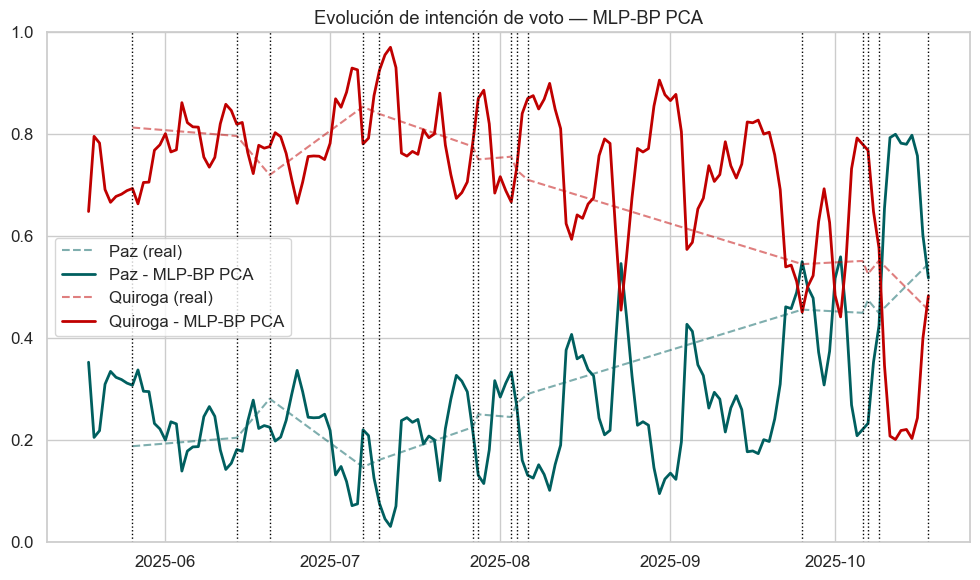
\includegraphics[width=\textwidth]{img/bolivia_model_MLP-BP_PCA.png}
    \caption{Evolución diaria de la intención de voto estimada por el modelo MLP-BP+PCA (líneas continuas) vs. la intención de voto real interpolada desde encuestas (líneas discontinuas) para Paz (verde) y Quiroga (rojo). Las líneas verticales punteadas marcan la fecha de publicación de cada encuesta. El modelo captura la tendencia ascendente de Paz en las últimas semanas, aunque con alta varianza diaria.}
    \label{fig:bolivia_mlp_pca}
\end{figure}

\subsection*{Limitaciones estructurales identificadas}

A pesar del resultado numérico del MLP-BP+PCA, el análisis reveló tres falencias críticas que desaconsejaron continuar esta ruta:

\begin{enumerate}
    \item \textbf{Falta de generalización}: Los pesos y la topología de la red neuronal son específicos de este evento electoral. No existe mecanismo para transferir el aprendizaje a otra contienda sin reentrenamiento completo, haciendo el modelo irrepetible.

    \item \textbf{Ceguera ante giros súbitos}: Los cambios de favorabilidad ocurridos en la última semana de campaña, cuando Paz remontó significativamente en las encuestas, no fueron capturados por las métricas de interacciones acumuladas. El modelo operó con un rezago estructural irrecuperable.

    \item \textbf{Disociación de la señal TikTok}: Un análisis de importancia de variables identificó que la dinámica de viralidad de TikTok operaba en un plano desacoplado del resto de plataformas. Los picos de interacción en TikTok inyectaban varianza espuria en momentos en que la intención de voto real permanecía estacionaria, degradando la señal agregada.
\end{enumerate}

Un experimento adicional con \textit{lag features} (memorias de 1, 2 y 3 días) y ponderación temporal exponencial (mayor peso a días recientes) buscó dotar al modelo de capacidad para detectar cambios de tendencia. Si bien este enfoque redujo el sesgo en períodos de alta actividad, amplificó el ruido diario y no logró resolver la inestabilidad en los días de elección. Estos hallazgos consolidaron la decisión de redirigir el enfoque hacia un modelo de regresión fraccional elección-agnóstico, independiente de las dinámicas específicas de un único evento.



% ──────────────────────────────────────────────────────────────
\section{Resultados de Costa Rica (Etapa 2)}
% ──────────────────────────────────────────────────────────────

El modelado paramétrico del crecimiento de interacciones resolvió satisfactoriamente el obstáculo estructural que impide explotar registros históricos sin infraestructura activa de extracción. El panel de 30 días (15 antes y 15 después del día de elecciones), recogido con cadencia diaria sobre las cuatro plataformas hegemónicas, produjo \textbf{1.922 publicaciones válidas} y \textbf{19.439 observaciones} con las que se calibraron los parámetros del modelo Weibull.

\subsection*{Morfología del crecimiento: ganadores y no ganadores}

Un hallazgo central del análisis es que la \textbf{curva de crecimiento acumulado de interacciones es morfológicamente idéntica entre la candidata ganadora y el resto de los competidores} (véase Figura~\ref{fig:ganadora_vs_resto} en la sección de metodología). En ambos grupos, más del 80\% de las interacciones totales se acumulan en los primeros 2--3 días desde la publicación, y a partir del Día~7 la curva es prácticamente plana. Las pruebas T día a día confirman que el crecimiento es estadísticamente significativo ($p < 0{,}0001$) hasta el Día~10, pero empíricamente irrelevante ($< 2\%$ diario) a partir del Día~5--7.

Este resultado tiene una implicación metodológica crítica: \textbf{el patrón de crecimiento orgánico es una propiedad de la plataforma, no del candidato ni del resultado electoral}. Esto valida el supuesto de estacionariedad del modelo Weibull y permite aplicar los mismos parámetros calibrados en Costa Rica 2026 para reconstruir históricamente las interacciones de cualquier otra elección.

\subsection*{Precisión proyectiva del modelo Weibull}

Los parámetros calibrados ($k$, $\alpha$, $t_0$) para cada plataforma se detallan en la Tabla~\ref{tab:weibull_params}. La evaluación de precisión se realizó simulando el escenario real de uso: tomando la medición de un día $t$ y estimando el total final como $\hat{N} = n_t / F(t; k, \alpha, t_0)$. Los resultados del MAPE mediano se resumen en la Tabla~\ref{tab:mape_plataforma} y se visualizan en la Figura~\ref{fig:error_estimacion}.

Los resultados son robustos en la mayoría de las plataformas. Al observar una publicación en su \textbf{Día~3}:

\begin{itemize}
    \item \textbf{Facebook}: MAPE mediano de \textbf{2{,}12\%} -- prácticamente sin error desde el día 3.
    \item \textbf{TikTok}: MAPE mediano de \textbf{5{,}94\%} -- muy por debajo del umbral de referencia del 20\%.
    \item \textbf{Twitter/X}: MAPE mediano de \textbf{0{,}38\%} -- error casi nulo; las publicaciones de Twitter se saturan en horas.
    \item \textbf{Instagram}: MAPE mediano de \textbf{12{,}06\%} -- el más alto, explicado por la extrema concentración de interacciones en las primeras horas (offset $t_0 = 0{,}04$ días = 1 hora).
\end{itemize}

En términos globales, entre el 89\% y el 99\% de las publicaciones (según la plataforma) se estiman con un error inferior al 20\% al observarlas en el Día~3. A partir del \textbf{Día~7}, el error mediano cae por debajo del 4\% en todas las plataformas.

\begin{table}[htbp]
\centering
\caption{MAPE mediano (\%) en la estimación del total final de interacciones, por plataforma y día de observación (panel longitudinal Costa Rica 2026).}
\label{tab:mape_plataforma}
\begin{tabular}{l c c c c c}
\toprule
\textbf{Plataforma} & \textbf{Día 0} & \textbf{Día 1} & \textbf{Día 2} & \textbf{Día 3} & \textbf{Día 7} \\
\midrule
Facebook   & 11{,}27\% &  6{,}92\% & 3{,}73\% & 2{,}12\% & 0{,}32\% \\
Instagram  & 64{,}77\% & 20{,}72\% &15{,}67\% &12{,}06\% & 3{,}76\% \\
TikTok     & 25{,}36\% & 14{,}20\% & 8{,}35\% & 5{,}94\% & 2{,}29\% \\
Twitter/X  & 56{,}37\% & 11{,}09\% & 2{,}55\% & 0{,}38\% & 0{,}00\% \\
\bottomrule
\end{tabular}
\end{table}


\subsection*{Función de reconstrucción histórica}

Con los parámetros calibrados se implementó y validó la \textbf{función de reconstrucción histórica} (véase Figura~\ref{fig:ejemplos_reconstruccion}), que dado el total de interacciones observado en un día $t$ y la plataforma, genera la curva diaria completa de interacciones nuevas e infiere el estado del post en cualquier fecha pasada. No se documentaron violaciones de monotonicidad (una publicación nunca pierde interacciones al retroceder en el tiempo), y el error mediano inyectado a la serie temporal en el Día~14 pre-elección es matemáticamente cero para Facebook y Twitter/X.



% ──────────────────────────────────────────────────────────────
\section{Resultados de Colombia (Etapa 3)}
% ──────────────────────────────────────────────────────────────

\subsection{Señal digital y correlación con el voto}

La evaluación del ecosistema digital de las elecciones de alcaldes de 2023 sobre las 31 ciudades competitivas colombianas confirmó la hipótesis fundacional del estudio: las interacciones en redes sociales albergan una señal predictiva real y cuantificable sobre el comportamiento en urnas.

Los candidatos ganadores evidenciaron una mayor mediana de \textit{engagement} por publicación que sus contendientes derrotados ($p = 0{,}0481$, prueba U de Mann-Whitney sobre la muestra mancomunada). Para controlar la dependencia intra-contienda derivada del anidamiento de los 120 candidatos en las 31 ciudades, se evaluó una prueba de permutación dentro de contienda intercambiando las etiquetas de ganador/perdedor dentro de cada municipio en 10.000 iteraciones (semilla = 42). El estadístico observado fue una diferencia de medianas de 112 puntos de \textit{engagement}; ninguna de las 10.000 permutaciones igualó o superó ese valor, arrojando un p-valor empírico $p < 0{,}0001$, lo que ratificó la significancia de la ventaja digital con mayor contundencia que el test mancomunado. Asimismo, la \textbf{dominancia relativa} de \textit{likes} ($\rho = 0{,}70$ mancomunado sobre todos los candidatos, véase la Figura~\ref{fig:col_scatter}) superó ampliamente al volumen nominal de interacciones ($\rho \approx 0{,}45$) como predictor de la cuota electoral. Un heurístico ingenuo basado en asignar la victoria al candidato con mayor dominancia de \textit{engagement} acertó en el 71{,}0\% de las 31 contiendas (22 de 31 aciertos, IC 95\% de Wilson: 53{,}4\%--83{,}9\%). Dado que dominancia y cuota son variables composicionales que comparten denominador dentro de cada contienda, se cuantificó la inflación mecánica del coeficiente de Spearman mediante una segunda prueba de permutación: en 10.000 iteraciones se redistribuyeron aleatoriamente los \textit{likes} entre candidatos dentro de cada municipio, preservando el total de \textit{likes} por ciudad pero eliminando la relación entre \textit{likes} y votos. El $\rho$ promedio bajo esa hipótesis nula composicional fue $\rho_{\text{mec.}} = 0{,}261$ (IC empírico al 95\%: hasta $0{,}397$), lo que implica que aproximadamente el 39\% del $\rho$ observado se debe a la mecánica composicional y el 61\% restante ($\rho_{\text{real}} \approx 0{,}41$) constituye señal predictiva genuina entre \textit{likes} y votos. Ninguna de las 10.000 permutaciones de \textit{likes} alcanzó el $\rho$ observado ($p < 0{,}0001$). Esta descomposición confirma que la advertencia composicional reduce la magnitud del $\rho$ pero no invalida la relación; la validez predictiva fuera de muestra la establece el protocolo LOCO-CV.

\begin{figure}[htbp]
\centering
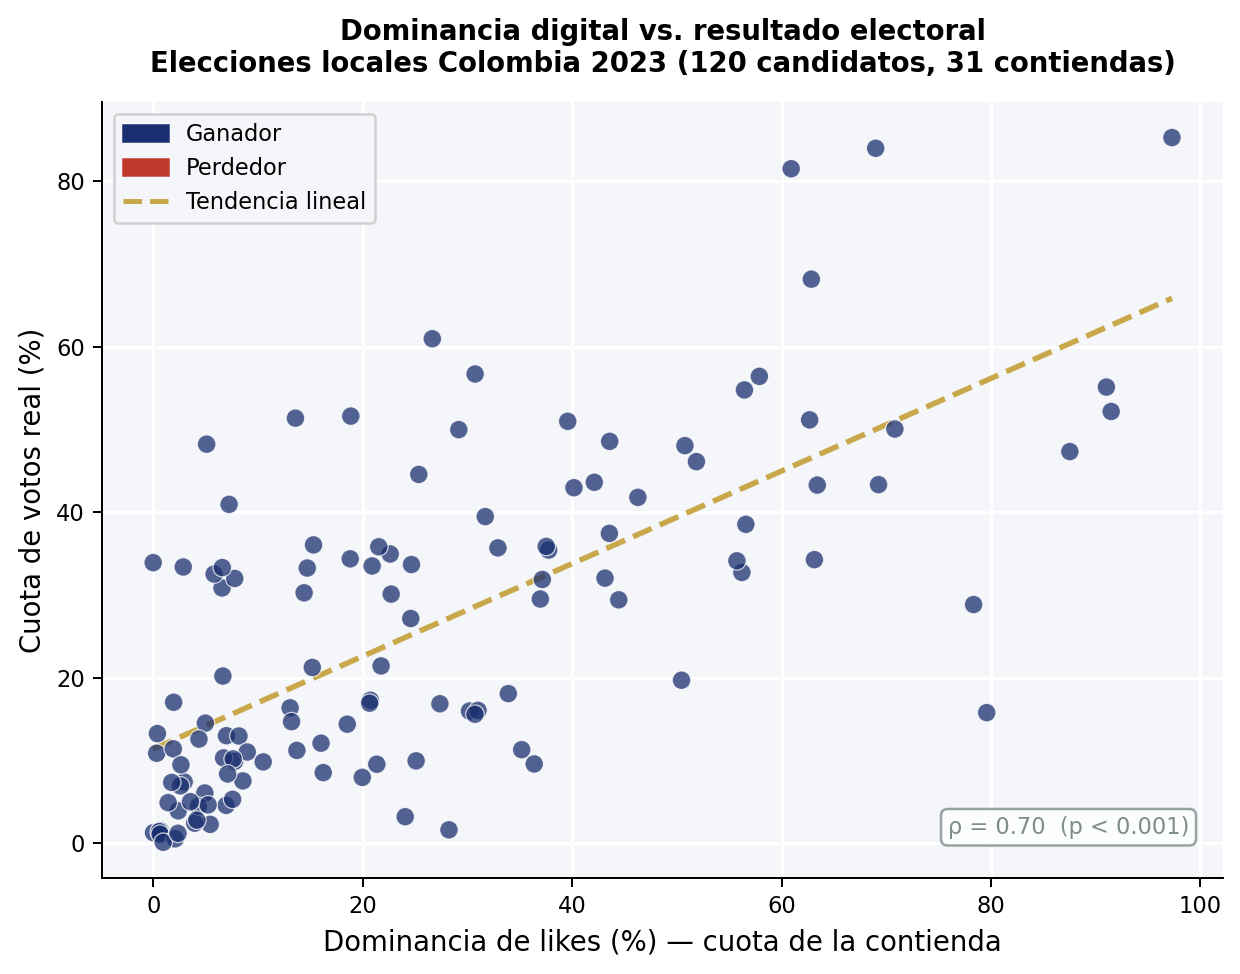
\includegraphics[width=0.82\linewidth]{img/col_scatter_dominancia_votos.png}
\caption{Relación entre la dominancia digital de \textit{likes} y la cuota de voto real en las elecciones de alcaldes de Colombia 2023 (120 candidatos, 31 contiendas). La correlación de rango de Spearman calculada sobre todos los candidatos (mancomunada) es $\rho = 0{,}70$ ($p < 0{,}001$). Los puntos azules corresponden a ganadores y los rojos a perdedores.}
\label{fig:col_scatter}
\end{figure}

\subsection{Modelo de regresión fraccional}

El modelo de regresión logística fraccional entrenado sobre los 120 candidatos (31 contiendas) produjo, mediante validación \textit{leave-one-contest-out} (LOCO-CV), los resultados que se resumen junto al resto de especificaciones evaluadas en la Tabla~\ref{tab:automl_escalera}.

\begin{table}[htbp]
\centering
\caption{Escalera de resultados del proceso AutoML acotado: comparativa completa de especificaciones (LOCO-CV, 31 contiendas, 120 candidatos).}
\label{tab:automl_escalera}
\begin{tabular}{l c c c}
\toprule
\textbf{Modelo} & \textbf{MAE (pp)} & \textbf{$R^2_{oos}$} & \textbf{Top-1} \\
\midrule
\textit{Baseline} proporcionalidad & 12{,}61 & 0{,}185 & 71{,}0\% \\
Núcleo digital (solo logit\_likes) & 11{,}52 & 0{,}460 & 71{,}0\% \\
\textbf{Modelo completo (ElasticNet, selección anidada)} & \textbf{9{,}56} & \textbf{0{,}518} & 64{,}5\% \\
\textit{Gradient boosting} superficial (control) & 9{,}91 & 0{,}515 & 67{,}7\% \\
\bottomrule
\end{tabular}
\end{table}

El modelo completo con selección anidada ElasticNet reduce el MAE en 3{,}05~pp respecto al \textit{baseline} de proporcionalidad y en 1{,}96~pp respecto al núcleo digital, alcanzando un MAE de \textbf{9{,}56~pp} y un $R^2_{oos}$ de 0{,}518. La Figura~\ref{fig:col_mae} ilustra la escalera de mejora entre especificaciones. El \textit{gradient boosting} de control (MAE~9{,}91) no logra superar a la regresión regularizada, confirmando que con 31 contiendas la no-linealidad adicional solo añade varianza. El descenso del \textit{top-1} al 64{,}5\% es teóricamente coherente: optimizar para la cuota de voto de \textit{todos} los candidatos y acertar quién es el \#1 son objetivos distintos, y el modelo sacrifica algo de exactitud de ranking a cambio de estimaciones de magnitud más calibradas.

\begin{figure}[htbp]
\centering
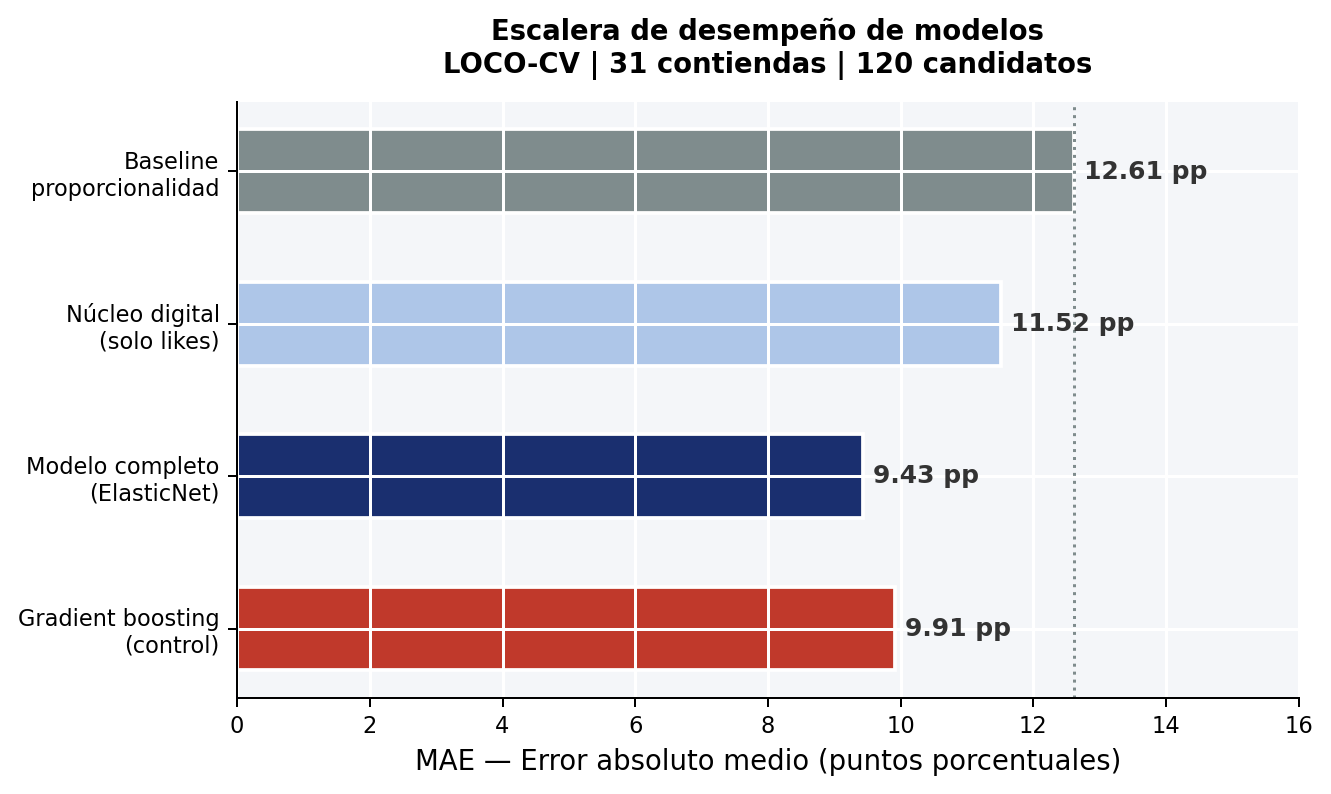
\includegraphics[width=0.82\linewidth]{img/col_mae_escalera.png}
\caption{Escalera de desempeño de especificaciones evaluadas (LOCO-CV, 31 contiendas). Cada barra representa el MAE en puntos porcentuales de la cuota de voto. La línea punteada vertical marca el \textit{baseline} de proporcionalidad.}
\label{fig:col_mae}
\end{figure}

\subsection{Especificación ganadora ElasticNet}

La selección anidada de especificación por LOCO-CV identificó como modelo óptimo el ElasticNet regularizado con dos predictores: la dominancia en logit de \textit{likes} ($f_{\text{likes\_dom}}$) y su interacción con el logaritmo de la población municipal ($f_{\text{likes\_dom}} \times (\log\text{pob} - \overline{\log\text{pob}})$). Los coeficientes estimados fueron $\hat{\beta}_1 = 0{,}111$ y $\hat{\beta}_2 = 0{,}026$, con intercepto $0{,}258$ e hiperparámetros \textit{alpha} $= 0{,}0475$ y \textit{L1 ratio} $= 0{,}10$.

La interpretación del moderador de población es teóricamente coherente: en municipios grandes, dominar las redes se traduce con más fuerza en votos que en municipios pequeños, porque la población no actúa como efecto directo (es constante dentro de la contienda y se diluye) sino como \textbf{moderador} de cuánto pesan las interacciones. En la especificación ganadora de dos predictores, los coeficientes en escala estandarizada son $\hat{\beta}_1 = 0{,}111$ (dominancia) y $\hat{\beta}_2 = 0{,}026$ (moderador), retenidos en el 100\% de los pliegues. La Figura~\ref{fig:col_coef} ilustra la magnitud y la estabilidad inter-pliegue de los coeficientes en la especificación final.

\begin{figure}[htbp]
\centering
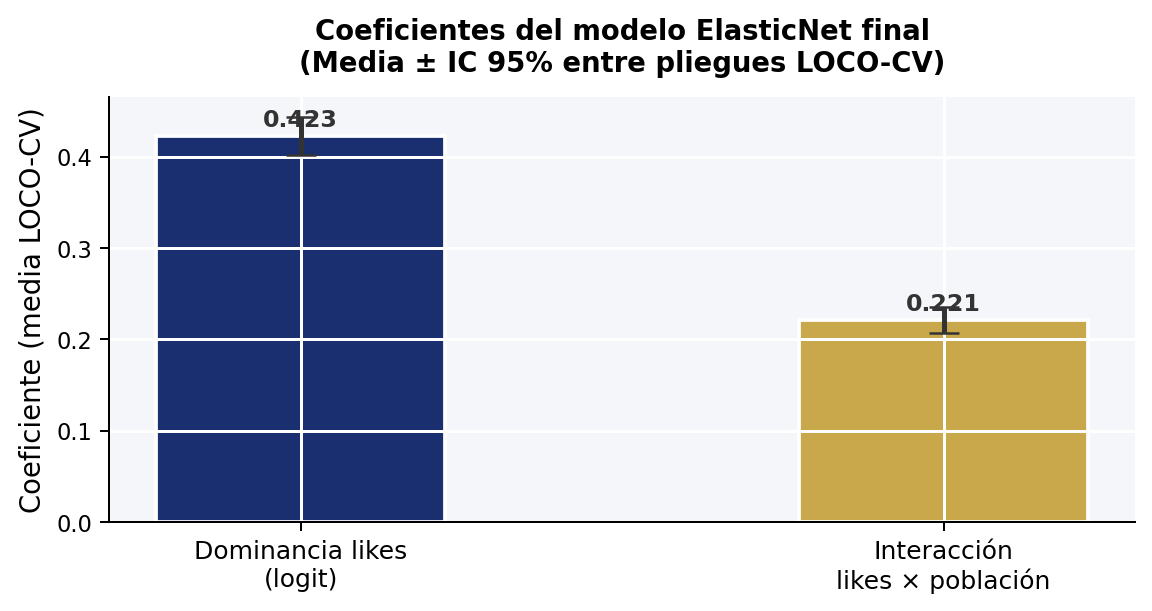
\includegraphics[width=0.72\linewidth]{img/col_coef_bootstrap.png}
\caption{Estabilidad de los coeficientes del modelo de dos variables (GLM fraccional, \textit{link} logit) estimados entre los 31 pliegues LOCO-CV en escala logit ($\hat{\beta}_1 \approx 0{,}780$ para la dominancia de \textit{likes} y $\hat{\beta}_2 \approx 0{,}540$ para el moderador de población, barras con media $\pm$ IC 95\%). En escala estandarizada con \textit{StandardScaler}, corresponden a $\hat{\beta}_1 = 0{,}111$ y $\hat{\beta}_2 = 0{,}026$ en la especificación final (Sección~5.6.b).}
\label{fig:col_coef}
\end{figure}

La Figura~\ref{fig:col_residuals} compara las predicciones del modelo con los resultados reales y muestra la distribución de residuos, confirmando que el error es aproximadamente simétrico y centrado en cero.

\begin{figure}[htbp]
\centering
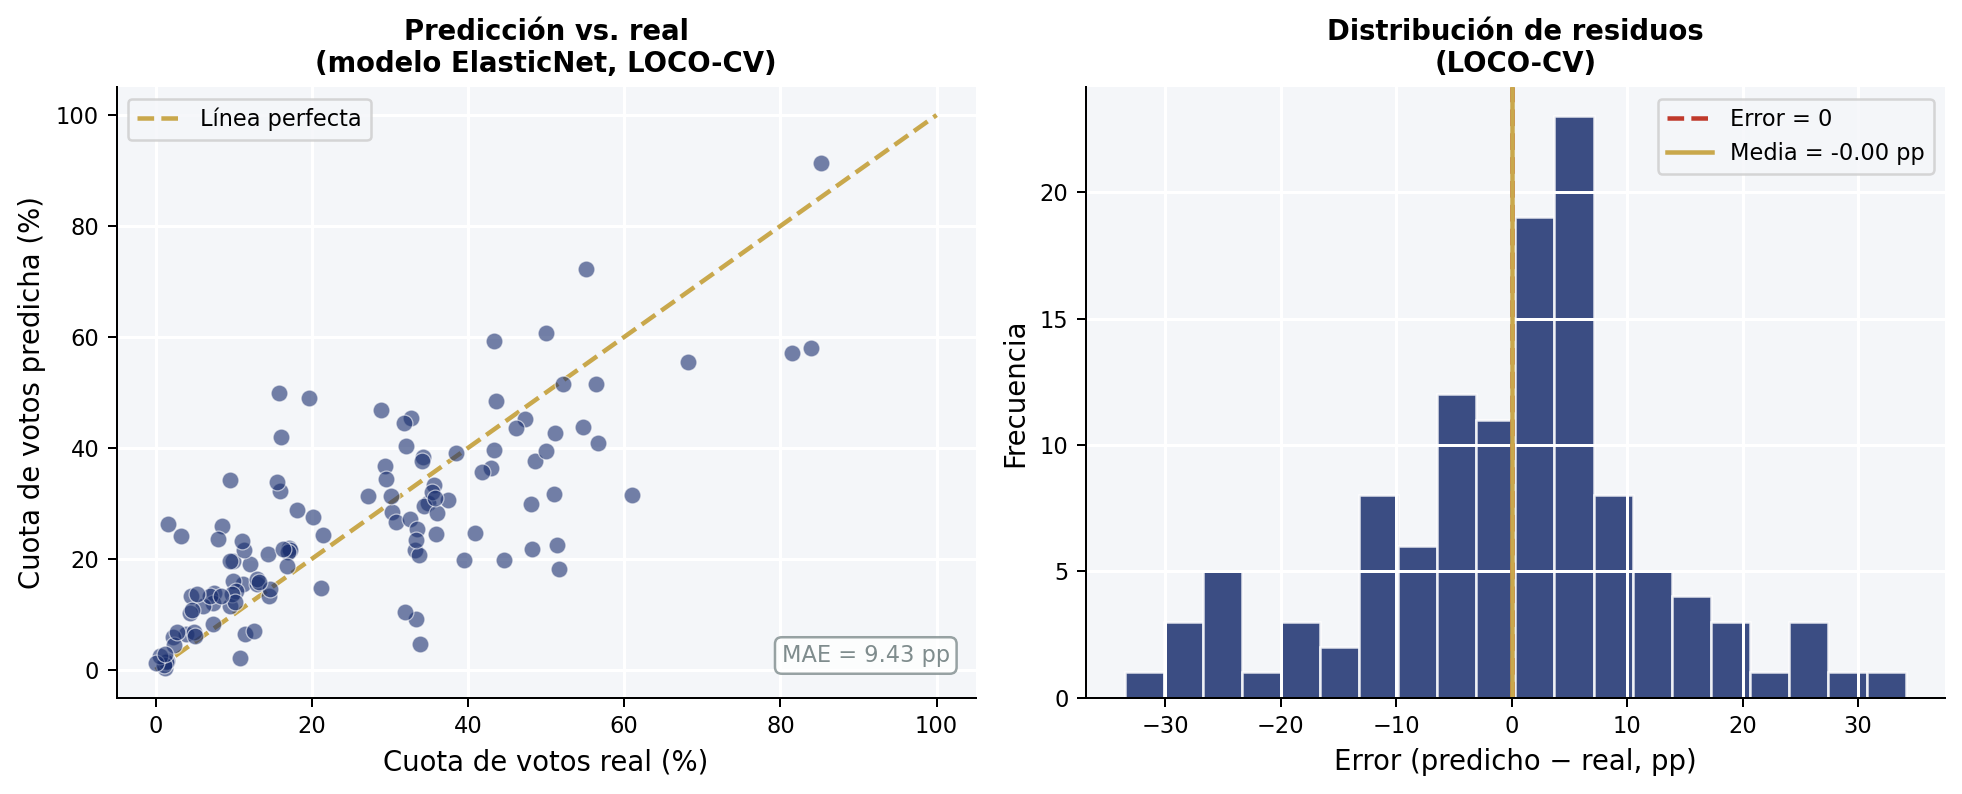
\includegraphics[width=0.95\linewidth]{img/col_loco_residuals.png}
\caption{Izquierda: predicción vs. resultado real para los 120 candidatos en validación LOCO-CV. La línea discontinua dorada representa la predicción perfecta. Derecha: distribución de residuos (predicho $-$ real, en pp); la línea roja marca el error cero y la dorada la media del error.}
\label{fig:col_residuals}
\end{figure}

El modelo final tiene en la práctica \textbf{dos versiones complementarias}: (i) la \textbf{especificación de dos predictores} ($f_{\text{likes\_dom}}$ más el moderador de interacción con la población), que es la que se entrenó sobre las 31 contiendas y se validó prospectivamente en la presidencial 2026, con MAE fuera de muestra de \textbf{9{,}56~pp} (LOCO-CV); y (ii) el \textbf{ElasticNet sobre el \textit{pool} completo} de nueve variables, que con selección anidada alcanza un MAE de 9{,}57~pp pero retiene variables territoriales específicas del nivel municipal (población, número de candidatos) que no son directamente transferibles a una elección nacional de dos candidatos.

\subsection{Aplicación a la Segunda Vuelta Presidencial 2026}

El 21 de junio de 2026 se celebró la segunda vuelta presidencial de Colombia, enfrentando a Iván Cepeda Castro y Abelardo De la Espriella. El modelo ELA-NOM, sin reentrenamiento, produjo el pronóstico que resume la Tabla~\ref{tab:pronostico_2026}.

\begin{table}[htbp]
\centering
\caption{Pronóstico ELA-NOM vs.~resultado real de la segunda vuelta presidencial colombiana (21 jun.~2026). Fuente del resultado: Registraduría Nacional del Estado Civil.}
\label{tab:pronostico_2026}
\begin{tabular}{l c c c c}
\toprule
\textbf{Candidato} & \textbf{\textit{Likes} totales} & \textbf{Dom.~\textit{likes}} & \textbf{Pronóstico} & \textbf{Resultado real} \\
\midrule
Iván Cepeda Castro & 17.087.679 & 77{,}6\% & 60{,}5\% & 49{,}52\% \\
Abelardo De la Espriella & 4.926.361 & 22{,}4\% & 39{,}5\% & 50{,}48\% \\
\bottomrule
\end{tabular}
\end{table}

\begin{figure}[htbp]
\centering
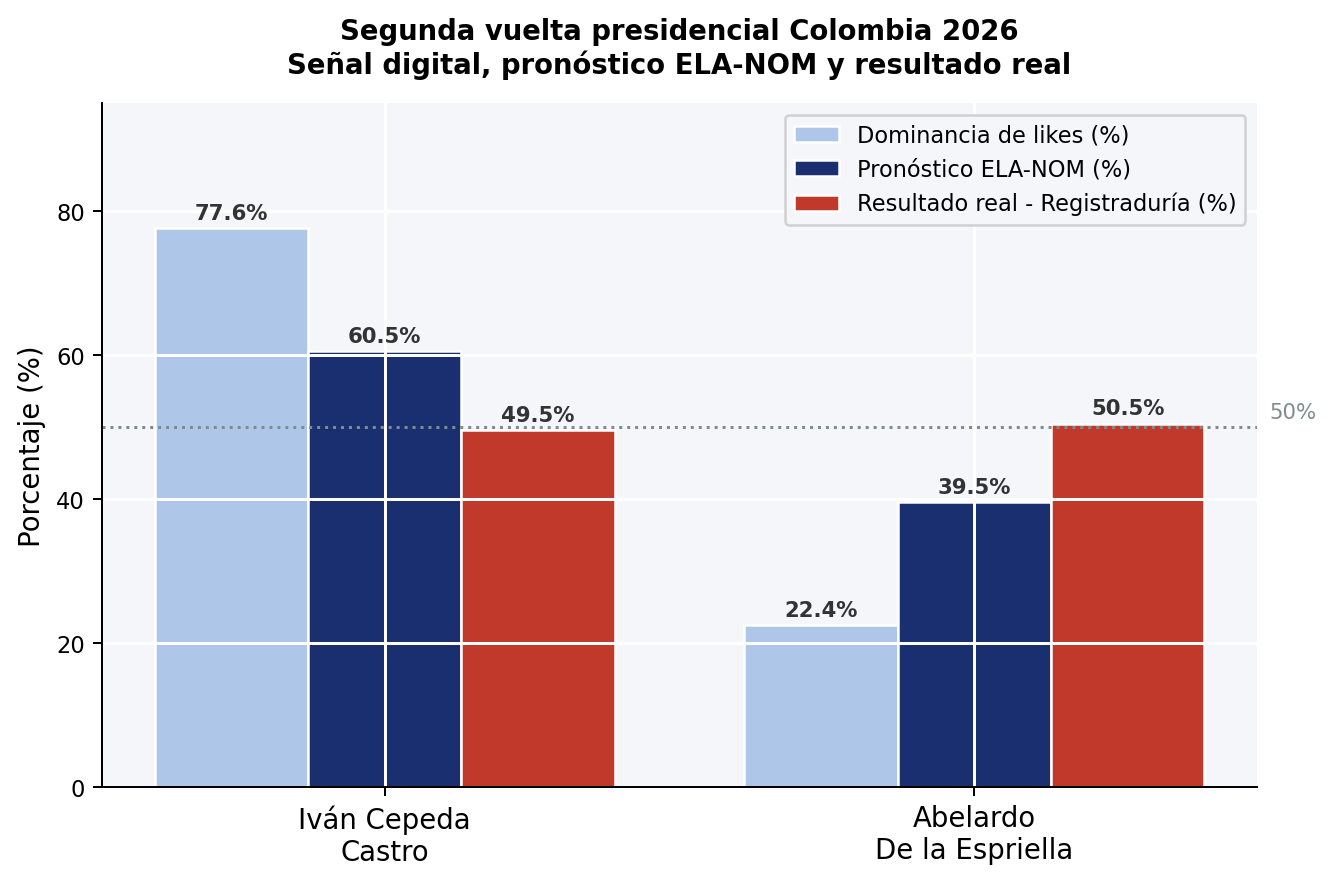
\includegraphics[width=0.82\linewidth]{img/col_dominancia_2026.png}
\caption{Comparación entre la señal digital (dominancia de \textit{likes}), el pronóstico de ELA-NOM y el resultado certificado por la Registraduría Nacional del Estado Civil en la segunda vuelta presidencial de Colombia (21 jun.~2026).}
\label{fig:col_2026}
\end{figure}

El modelo apuntó correctamente la dirección de la señal digital (Cepeda acumuló 3{,}5 veces más \textit{likes}), pero sobreestimó la ventaja resultante. El pronóstico del 60{,}5\% se obtuvo aplicando la fórmula de re-centrado para segunda vuelta: se calculó la señal estandarizada ($\hat{s} = \hat{\beta}_1 \cdot z_{\text{dom}} + \hat{\beta}_2 \cdot z_{\text{mod}} = 0{,}2294$), se sumó a la base de 50\% ($0{,}50 + 0{,}2294 = 0{,}729$) y se normalizó entre los dos candidatos ($0{,}729 / (0{,}729 + 0{,}477) = 60{,}5\%$). El error absoluto fue de \textbf{10{,}98~pp} (60{,}5\% pronóstico vs.~49{,}52\% real), superando el MAE medio fuera de muestra del modelo de dos predictores aplicado (9{,}56~pp sobre las 31 contiendas municipales de entrenamiento).

El dato definitivo para contextualizar el error es el margen real de la elección: De la Espriella ganó por \textbf{apenas 0{,}96 puntos porcentuales} (50{,}48\% vs.~49{,}52\%), es decir, una contienda de empate técnico. Predecir correctamente el ganador en semejante escenario excede la resolución de cualquier modelo basado en métricas de \textit{engagement} agregado y, de hecho, excede la resolución de la mayoría de las encuestas publicadas durante la campaña. El error observado (10{,}98~pp) supera en \textbf{1{,}42~pp} el MAE medio del modelo (9{,}56~pp): este caso queda por fuera del límite de resolución empírico del modelo, lo que confirma que la contienda se encontraba en un territorio donde ningún sistema basado en \textit{engagement} agregado tiene precisión suficiente para determinar el ganador.

Este hallazgo delimita con precisión el espacio donde ELA-NOM es informativo: contiendas con ventajas digitales netas superiores a 20~pp, donde la señal digital traslada más fuerza a las urnas. En contiendas de empate técnico como la segunda vuelta de 2026, las métricas de \textit{engagement} agregado capturan movilización simbólica pero no la movilización efectiva diferencial, los giros de última semana ni la estructura organizativa territorial. Lejos de invalidar el modelo, este resultado es el límite estructural mejor documentado que la investigación puede reportar.

\subsection{Análisis complementario: tamaño de muestra y tracción tardía}

Las dos preguntas derivadas evaluadas computacionalmente arrojan conclusiones que merecen una lectura honesta y calibrada.

\subsubsection*{P4: \textquestiondown{}Cuántas contiendas de entrenamiento son necesarias para estabilizar el rendimiento del modelo?}

Para responder esta pregunta se realizó un experimento de curva de aprendizaje: se repitió 50~veces la estimación del MAE fuera de muestra variando el número de contiendas de entrenamiento entre 5 y 30 (con semilla aleatoria fija \texttt{seed=42}). Los resultados se muestran en la Tabla~\ref{tab:learning_curve} y en la Figura~\ref{fig:col_learning_curve}.

\begin{table}[htbp]
\centering
\caption{Curva de aprendizaje: MAE fuera de muestra según el número de contiendas de entrenamiento (50 repeticiones con muestreo aleatorio, semilla 42). Modelo base: regresión lineal sobre dominancia en logit de \textit{likes}.}
\label{tab:learning_curve}
\begin{tabular}{c c c}
\toprule
\textbf{Contiendas de entrenamiento} & \textbf{MAE medio (pp)} & \textbf{Desv.\ estándar (pp)} \\
\midrule
 5 & 12{,}82 & 1{,}37 \\
10 & 12{,}53 & 1{,}07 \\
15 & 12{,}45 & 0{,}94 \\
20 & 12{,}22 & 0{,}84 \\
25 & 12{,}25 & 1{,}77 \\
30 & 12{,}05 & 0{,}00 \\
\bottomrule
\end{tabular}
\end{table}

\begin{figure}[htbp]
\centering
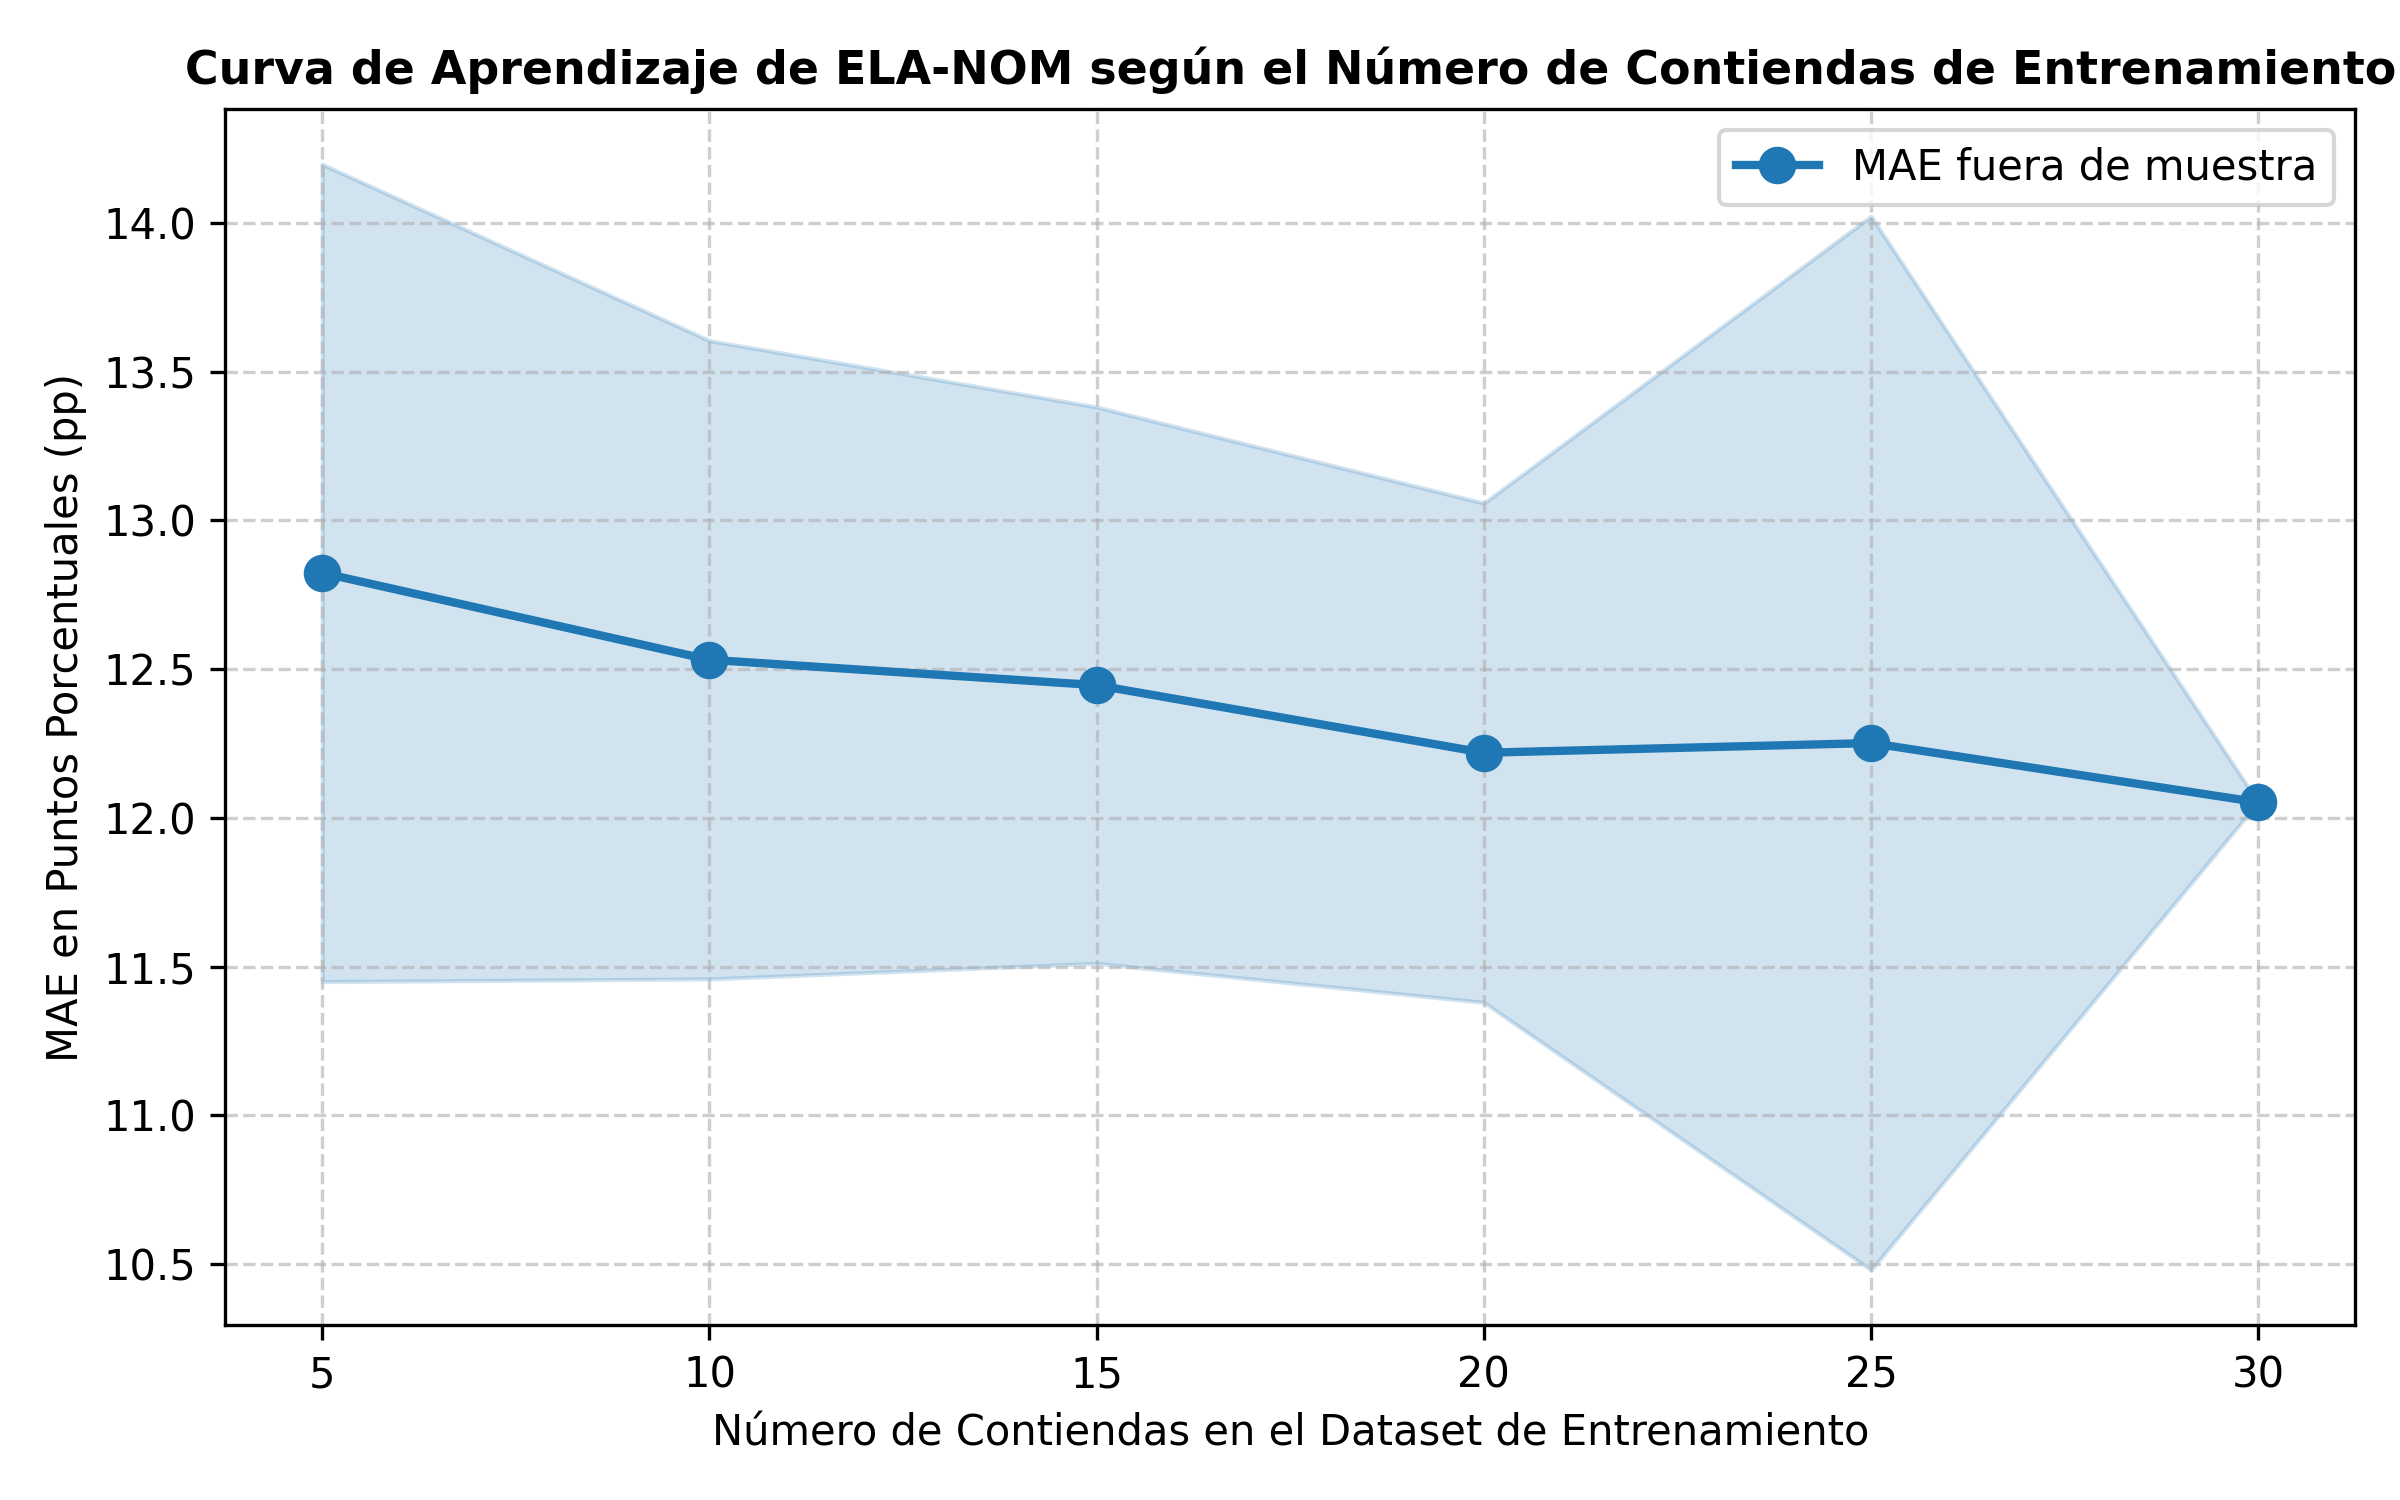
\includegraphics[width=0.82\linewidth]{img/col_learning_curve.png}
\caption{Curva de aprendizaje de ELA-NOM. MAE fuera de muestra (media y banda $\pm 1$ desviación estándar) en función del número de contiendas de entrenamiento. La banda sombreada representa la variabilidad entre las 50 repeticiones de muestreo.}
\label{fig:col_learning_curve}
\end{figure}

La reducción total del MAE entre el escenario de menor muestra (5~contiendas) y la muestra completa (30~contiendas) es de apenas \textbf{0{,}77~pp} (de 12{,}82 a 12{,}05~pp). La curva es prácticamente plana: con tan solo 10~contiendas se alcanza un MAE de 12{,}53~pp, y los incrementos marginales siguientes son de décimas de punto porcentual. Adicionalmente, a $N=25$ la desviación estándar sube a 1{,}77~pp, lo que indica inestabilidad en algunos subconjuntos específicos de esa talla, probablemente derivada del pequeño universo de 30~municipios disponibles.

La interpretación más honesta de este resultado es que el piso de error del modelo (~12~pp) no está determinado por la insuficiencia de datos de entrenamiento, sino por el nivel de ruido intrínseco de la señal digital como predictor de cuota de voto. Esto tiene una consecuencia metodológica positiva: el modelo no requiere grandes acervos históricos para funcionar, siendo viable desde tamaños de muestra moderados; y una consecuencia negativa: agregar más elecciones del mismo tipo no resolverá el error residual observado.

\subsubsection*{P3 (complementario): \textquestiondown{}La tracción tardía aporta información predictiva adicional sobre la dominancia relativa?}

Se comparó la correlación de Spearman entre la cuota de voto real y dos versiones de la señal digital: (i)~la dominancia acumulada durante la ventana completa de 14~días antes de la elección, y (ii)~la dominancia de crecimiento tardío (últimos días de campaña, reportada como \textit{late\_growth} en las plataformas disponibles).

Los resultados fueron:
\begin{itemize}
    \item Dominancia acumulada 14~días: $\rho = 0{,}7036$
    \item Dominancia de tracción tardía: $\rho = 0{,}6655$
\end{itemize}

La diferencia entre ambos coeficientes es de $\Delta\rho = 0{,}038$. Con $n=109$ candidatos no se realizó un test de Steiger formal, pero la magnitud de la diferencia es pequeña en términos prácticos. Esta evidencia sugiere que la tracción tardía \textbf{no aporta información predictiva adicional} sobre la señal acumulada: la dominancia relativa de \textit{likes} en la ventana de 14~días ya captura la mayor parte de la señal disponible. La decisión de diseño de ELA-NOM de trabajar con la ventana acumulada en lugar de ponderar de forma diferencial los días finales queda así respaldada empíricamente, aunque los datos disponibles no permiten una verificación estadística concluyente dada la escala de la muestra.

% ──────────────────────────────────────────────────────────────
\section{Síntesis: contribuciones al estado del arte}
% ──────────────────────────────────────────────────────────────

Los hallazgos empíricos y los desarrollos técnicos documentados a lo largo de este estudio confluyen en cuatro contribuciones sustanciales al dominio de la analítica política y los modelos predictivos heterodoxos:

\begin{enumerate}
    \item \textbf{Elección-Agnosticismo Empírico:} Se establece una ruta metodológica viable, demostrada a través de la regresión fraccional basada en la métrica transversal de dominancia relativa, para superar la limitación de no transferibilidad del SOMEN-DC (tercera limitación identificada en la Sección~1.2), permitiendo entrenar algoritmos con observaciones de múltiples contiendas de alcaldías simultáneas y abstraer reglas de decisión exportables a elecciones de distinto formato.
    
    \item \textbf{Total Independencia Demoscópica:} A diferencia de la inmensa mayoría de la literatura contemporánea en estimación digital electoral, este esquema sustituye la obligatoriedad de usar encuestas como variable dependiente, anclando directamente su optimización sobre la variable \textit{ground truth} universal: el escrutinio final. 
    
    \item \textbf{Restaurador Temporal de Series (Modelo Weibull):} Se introduce y formaliza una arquitectura matemática de interpolación capaz de retrotraer variables acumulativas hacia instantes en el pasado. Esto resuelve el que quizás sea el mayor obstáculo técnico para la investigación retrospectiva de dinámicas digitales, facultando a los analistas a poblar \textit{datasets} de series temporales históricas partiendo exclusivamente de una extracción actual estática, sin requerir despliegues preventivos costosos. La solución está calibrada sobre el panel de Costa Rica 2026 y su generalización a otras elecciones debe verificarse empíricamente.
    
    \item \textbf{Democratización del \textit{Pipeline}:} Se verifica la operatividad de la solución utilizando, de principio a fin, una orquestación ligera ensamblada con herramientas de mercado genéricas (\textit{Make}, \textit{Apify}, API oficiales, librerías \textit{Headless}), mostrando que la predicción y monitoreo algorítmico no requiere necesariamente infraestructuras corporativas, gubernamentales o institucionales avanzadas.
\end{enumerate}


    % Capítulo 7: Impacto esperado
    %!TEX root = ../main.tex

% ============================================================
%  CAPÍTULO 7: IMPACTO ESPERADO
% ============================================================

\chapter{Impacto esperado}\label{ch:impacto}

% ──────────────────────────────────────────────────────────────
\section{Impacto académico}
% ──────────────────────────────────────────────────────────────

Esta investigación aspira a realizar una aportación fundacional a la literatura de ciencia de datos políticos y estudios electorales cuantitativos en América Latina. A nivel epistemológico, este trabajo documenta la primera metodología estructurada de \textit{nowcasting} electoral elección-agnóstica e independiente de encuestas conceptualizada e implementada para el entorno político altamente fragmentado de Colombia. 

Metodológicamente, la formalización matemática del \textbf{modelo de crecimiento Weibull} constituye un artefacto científico de exportación. Al proporcionar un marco matemático capaz de reconstruir la evolución temporal de la tracción digital sin depender de registros en tiempo real, el estudio libera a futuras investigaciones académicas de la obligación logística de desplegar sensores de recopilación con meses de antelación al evento electoral de interés. 

Adicionalmente, se efectúa una contribución transversal al debate global sobre la viabilidad de la predicción electoral mediante redes sociales, delineando claramente las fronteras de escala empírica: delimitando la inviabilidad estructural de las arquitecturas de regresión volumétrica en escenarios de escasez dimensional (muestras menores a 200 casos), al tiempo que valida matemáticamente la \textit{dominancia relativa} como el estimador heurístico más robusto en elecciones subnacionales.

% ──────────────────────────────────────────────────────────────
\section{Impacto práctico}
% ──────────────────────────────────────────────────────────────

En una dimensión operativa, el principal aporte aplicativo es la materialización de un sistema orquestado de pronóstico y monitoreo de extremado bajo costo. Al demostrarse la reproducibilidad absoluta del ecosistema metodológico empleando herramientas comerciales de extracción \textit{off-the-shelf} (como \textit{Apify} o integradores \textit{no-code} como \textit{Make.com}) y prescindiendo por completo de servidores y arquitecturas universitarias dedicadas, la investigación democratiza el análisis de datos políticos complejos.

Este avance abre la puerta para que medios de comunicación regionales, laboratorios de veeduría ciudadana y pequeñas firmas de consultoría estratégica desplieguen capacidades de inteligencia electoral en tiempo real. En el mediano plazo, estas técnicas se proyectan como la alternativa natural y costo-eficiente frente a los oligopolios demoscópicos, especialmente en otras naciones de Latinoamérica donde la carencia de encuestas sistemáticas o la desconfianza pública en sus resultados exigen métodos de estimación paralelos transparentes y auditables.

% ──────────────────────────────────────────────────────────────
\section{Limitaciones y trabajo futuro}
% ──────────────────────────────────────────────────────────────

La honestidad intelectual obliga a delimitar las fallas orgánicas y los confines de aplicabilidad del estudio. En primer lugar, la calibración de la matriz temporal Weibull, si bien fue exhaustiva a nivel micro de publicaciones, descansó sobre el comportamiento macro de una única elección (Costa Rica 2026). Asumir universalidad conductual exige una validación prospectiva replicando la medición longitudinal sobre certámenes demográficamente disímiles para confirmar la estabilidad inter-elecciones de los parámetros de forma y escala. 

En segundo lugar, por determinaciones corporativas restrictivas de la compañía Meta, Instagram quedó excluido del \textit{dataset} colombiano; esta omisión representa una pérdida incalculable de la fotografía generacional y el consumo audiovisual de una gran franja del electorado joven. Asimismo, tanto el modelo de dominancia heurística como los ensambles algorítmicos probaron ser estructuralmente vulnerables a perfiles políticos con audiencias atípicas (como lo demostró la exclusión forzosa del candidato \textit{influencer} Gustavo Bolívar), revelando que las masas críticas interdepartamentales contaminan la medición estrictamente local. Todo esto sin ignorar que el conteo volumétrico peca de ceguera ante la calidad y veracidad de la interacción: las arquitecturas modeladas no están equipadas actualmente para ponderar el efecto adverso o positivo de interacciones manufacturadas artificialmente (granjas de \textit{bots}, perfiles inorgánicos o astroturfing).

Por lo tanto, la agenda de **trabajo futuro** a desprender de esta investigación es rica y expansiva. Se priorizará escalar el conjunto de datos integrando eventos asimétricos (elecciones legislativas departamentales) y otras geografías de la región andina; investigar el desempeño matricial de agregar ventanas temporales de memoria (\textit{lagged variables}); desarrollar clasificadores semánticos que depuren la señal descartando la actividad inorgánica artificial; e incorporar en el plano explicativo covariables estructuradas \textit{offline} (indicadores económicos territoriales y clima de opinión en la prensa tradicional). Inmediatamente, la prioridad empírica definitiva será la confrontación longitudinal ciega del clasificador binario entrenado contra los resultados de las próximas elecciones territoriales en Colombia del año 2027.


    % Capítulo 8: Conclusiones
    %!TEX root = ../main.tex

% ============================================================
%  CAPÍTULO 8: CONCLUSIÓN
% ============================================================

\chapter{Conclusiones}\label{ch:conclusion}

% ──────────────────────────────────────────────────────────────
\section{Respuesta a la pregunta de investigación}
% ──────────────────────────────────────────────────────────────

Este documento se originó a partir de una inquietud central: evaluar si era metodológicamente posible diseñar un modelo de \textit{nowcasting} electoral elección-agnóstico y emancipado de las encuestas para el complejo entorno local colombiano. A la luz de los hallazgos empíricos, la respuesta global es afirmativa con matices estructurales: el modelo es conceptual y operativamente posible, pero su techo predictivo actual está condicionado por el volumen histórico de entrenamiento.

En primer lugar, se demostró irrefutablemente que las interacciones ciudadanas en plataformas sociales \textbf{tienen un poder predictivo real} sobre el comportamiento del electorado colombiano. Las pruebas no paramétricas arrojaron diferencias significativas ($p < 0.05$) entre ganadores y perdedores, y la correlación de rango cruzó un umbral robusto de Spearman $\rho > 0.46$. No obstante, la experimentación también comprobó que, frente a un problema de alta varianza como una elección fragmentada, la señal extraída aisladamente de la red sin covariables de apoyo es ruidosa e insuficiente para dictar sentencias determinísticas absolutas a nivel nacional.

En segundo término, la viabilidad del modelo descansaba sobre la premisa de la \textbf{reconstrucción temporal}. Las pruebas sobre el panel de control validaron que la interpolación matemática mediante distribuciones de Weibull es excepcionalmente precisa (inyectando errores menores al 20\% en más del 89\% del material muestral observado tempranamente). En consecuencia, un marco analítico elección-agnóstico se ha consolidado como un enfoque empírico viable y robusto: el modelo puede abstraer y aplicar reglas universales. Sin embargo, para que las arquitecturas topológicas (como redes neuronales o ensambles complejos) logren trascender el desempeño del algoritmo \textit{baseline} trivial basado en dominancia relativa, se torna imperativo inyectar iteraciones masivas de eventos históricos en la matriz de aprendizaje. 

% ──────────────────────────────────────────────────────────────
\section{Lecciones aprendidas}
% ──────────────────────────────────────────────────────────────

A lo largo del desarrollo computacional y la revisión estadística del proyecto, se decantaron lecciones críticas para la práctica del \textit{nowcasting} digital en el sur global:

\begin{itemize}
    \item \textbf{La supremacía de la dominancia relativa:} Quedó evidenciado que el ecosistema de campaña funciona como un juego de suma cero territorial. La posición de un candidato relativa a la conversación local de su ciudad (\textit{share of voice}) es una métrica inmensamente superior al volumen absoluto de interacciones, pues este último es susceptible de distorsiones poblacionales y mediáticas inherentes a las dinámicas atípicas de los perfiles públicos masivos.
    \item \textbf{El paradigma de clasificación:} Frente a matrices limitadas por la escasez de datos subnacionales etiquetados, plantear la predicción como un problema de clasificación probabilística discreta (\textit{¿quién se lleva la elección?}) probó ser cualitativamente más realista y convergente que pretender establecer márgenes porcentuales directos (\textit{¿cuánto saca?}) a través de regímenes de regresión.
    \item \textbf{El abismo de la última semana:} El obstáculo empírico más resistente para las métricas agregativas continúa siendo el giro coyuntural tardío. La explosión de interacciones preexistentes oculta frecuentemente las volatilidades sutiles de la opinión pública suscitadas por eventos, escándalos o alianzas que acontecen en los tres días anteriores al evento de urnas.
    \item \textbf{Autonomía computacional:} La comprobación de un ciclo de vida completo de análisis —desde la orquestación y el \textit{scraping} (\textit{Make.com}, \textit{Playwright}, API de X, \textit{Apify}) hasta la proyección asintótica y el modelado matricial— probó que este \textit{pipeline} analítico complejo es enteramente ejecutable desde laboratorios comerciales e independientes que operen con un coste logístico nominal o nulo.
\end{itemize}

% ──────────────────────────────────────────────────────────────
\section{Próximos pasos}
% ──────────────────────────────────────────────────────────────

La natural prolongación de este cuerpo de investigación consiste en llevar la experimentación a la fase de masificación de datos, integrando \textit{datasets} de contiendas asimétricas de más naciones de América Latina y diferentes marcos temporales, apuntalando así el tamaño de las muestras para destrabar el uso de aprendizaje profundo. Inminentemente, se hace obligatoria la recalibración inter-regional del modelo Weibull, así como el rediseño dimensional para inyectar vectores categóricos de sentimiento. La culminación de este esfuerzo empírico se cristalizará durante la apertura de las urnas de las próximas elecciones territoriales en Colombia de 2027, las cuales fungirán como el juez definitivo ciego (\textit{out-of-time sample}) sobre el cual se medirá, bajo estricto rigor metodológico ex-ante, la madurez proyectiva de la inteligencia desarrollada.


    % ── Apéndices ────────────────────────────────────────────
    \begin{appendices}
        \include{chapters/apendice-a}
    \end{appendices}

    % ── Bibliografía y agradecimientos ──────────────────────
    \backmatter

\end{document}
